\documentclass[aspectratio=169,12pt,t]{beamer}

% --- Theme: Metropolis (modern, clean) ---
\usetheme[progressbar=frametitle,numbering=fraction,block=fill]{metropolis}

% --- Fira Sans font (install texlive-fonts-extra if missing) ---
\IfFileExists{FiraSans.sty}{\usepackage[sfdefault]{FiraSans}}{}

% --- Light background with warm accent ---
\definecolor{mDarkTeal}{RGB}{35,55,59}
\definecolor{mLightBrown}{RGB}{235,228,216}
\definecolor{mAccent}{RGB}{140,70,20}

\setbeamercolor{normal text}{fg=mDarkTeal,bg=white}
\setbeamercolor{alerted text}{fg=mAccent}
\setbeamercolor{frametitle}{bg=mDarkTeal,fg=white}
\setbeamercolor{progress bar}{fg=mAccent,bg=mLightBrown}
\setbeamercolor{title separator}{fg=mAccent}
\setbeamercolor{progress bar in head/foot}{fg=mAccent,bg=mLightBrown}
\setbeamercolor{progress bar in section page}{fg=mAccent,bg=mLightBrown}

% --- Packages ---
\usepackage[utf8]{inputenc}
\usepackage{amsmath,amssymb,amsthm}
\usepackage{mathrsfs}
\usepackage{tikz}
\usetikzlibrary{arrows.meta,positioning,calc,decorations.pathreplacing,shapes,patterns}
\usepackage{pgfplots}
\pgfplotsset{compat=1.18}

% --- TikZ diagram styles (shared across the series) ---
\tikzset{
  axisln/.style={-{Stealth[length=2.6mm]}, line width=0.8pt, gray!75},
  curveln/.style={line width=1.6pt, line cap=round, line join=round},
  projln/.style={dash pattern=on 2.6pt off 2pt, line width=0.7pt},
  guide/.style={-{Stealth[length=2.6mm,width=2.2mm]}, line width=1.1pt},
}
% point marker with a white halo: \dotpt{color}{(coord)}
\newcommand{\dotpt}[2]{%
  \fill[white] #2 circle (3.6pt);
  \fill[#1] #2 circle (2.4pt);
}
% open point marker: \opendotpt{color}{(coord)}
\newcommand{\opendotpt}[2]{%
  \fill[white] #2 circle (3.6pt);
  \draw[#1, line width=1pt] #2 circle (2.4pt);
}

% --- Semi-transparent white highlight for text on top of background images ---
\usepackage[most]{tcolorbox}

% Inline highlight: \hl{short text}
\newtcbox{\hl}{%
  nobeforeafter, tcbox raise base,
  colback=white, opacityback=0.6,
  colframe=white, opacityframe=0,
  sharp corners, boxsep=2pt, left=3pt, right=3pt, top=2pt, bottom=2pt%
}

% Block highlight: \begin{hlbox} ... \end{hlbox}  (multi-line, paragraphs, itemize)
% Optional argument accepts any tcolorbox key, e.g. [width=0.6\linewidth]
\newtcolorbox{hlbox}[1][]{%
  enhanced, breakable,
  colback=white, opacityback=0.6,
  colframe=white, opacityframe=0,
  boxsep=3pt, left=6pt, right=6pt, top=4pt, bottom=4pt,
  sharp corners,
  {#1}%
}

% --- Custom colors for content types ---
\definecolor{defcolor}{RGB}{25,85,120}
\definecolor{thmcolor}{RGB}{140,35,35}
\definecolor{proofcolor}{RGB}{35,100,50}
\definecolor{excolor}{RGB}{140,75,10}
\definecolor{remcolor}{RGB}{90,90,90}

% --- Beamer blocks for mathematical content types (semi-transparent) ---
\tcbset{hlblockbase/.style={
  enhanced, breakable,
  coltitle=white, fonttitle=\bfseries,
  opacitybacktitle=0.8, opacityback=0.6,
  opacityframe=0,
  sharp corners,
  boxsep=1pt, left=5pt, right=5pt, top=2pt, bottom=2pt,
  toptitle=1pt, bottomtitle=1pt,
  before upper={\setlength{\abovedisplayskip}{4pt}\setlength{\belowdisplayskip}{4pt}}
}}

\newtcolorbox{defblock}[1]{hlblockbase, title={#1},
  colbacktitle=defcolor, colback=defcolor!15, colframe=defcolor}
\newtcolorbox{thmblock}[1]{hlblockbase, title={#1},
  colbacktitle=thmcolor, colback=thmcolor!15, colframe=thmcolor}
\newtcolorbox{proofblock}[1]{hlblockbase, title={#1},
  colbacktitle=proofcolor, colback=proofcolor!15, colframe=proofcolor}
\newtcolorbox{exblock}[1]{hlblockbase, title={#1},
  colbacktitle=excolor, colback=excolor!15, colframe=excolor}
\newtcolorbox{remblock}[1]{hlblockbase, title={#1},
  colbacktitle=remcolor, colback=remcolor!15, colframe=remcolor}

% --- Metadata ---
\title{Chapter 7: Sequences and Series of Functions}
\subtitle{Section: Discussion of Main Problem}
\author{Based on Walter Rudin's \emph{Principles of Mathematical Analysis}}
\date{}

\begin{document}

{
\usebackgroundtemplate{%
  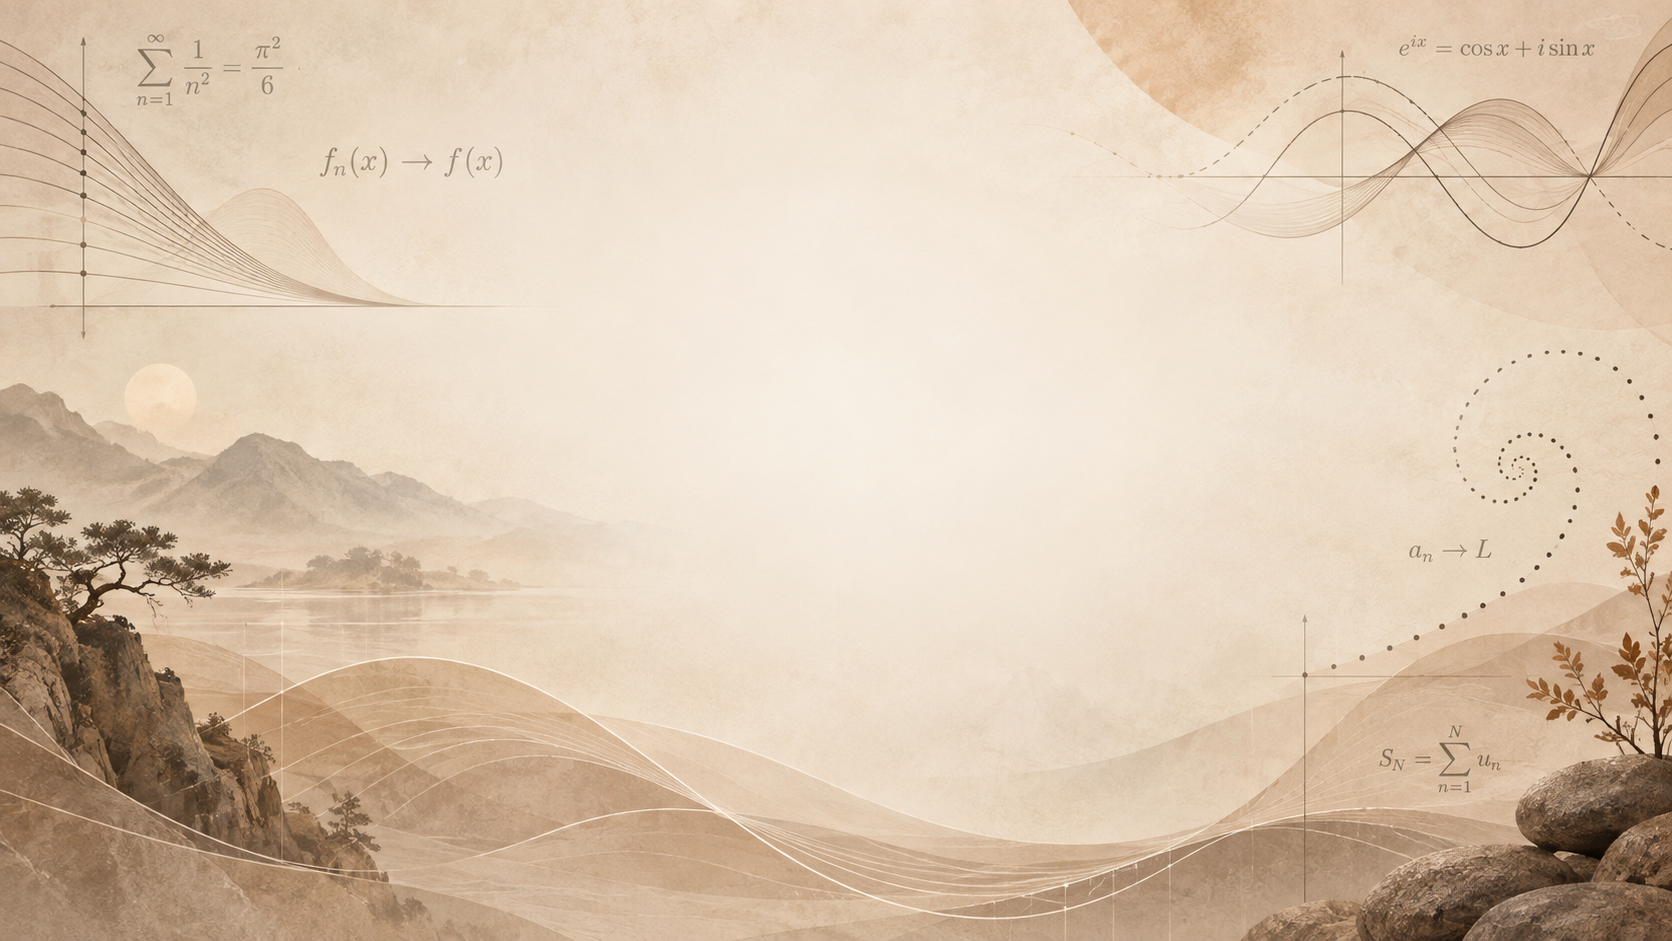
\includegraphics[width=\paperwidth,height=\paperheight,keepaspectratio=false]{chapter_07_bg_00.png}%
}
\begin{frame}[plain]
  \titlepage

  \note{
    Welcome to Chapter 7, Sequences and Series of Functions. This is
    the first section, Discussion of Main Problem. Up to now, the
    things that converged were numbers: sequences of real or complex
    numbers, or the values of a single function as its variable
    approaches a point. In this chapter the objects that converge are
    functions themselves. We have a whole sequence of functions "f"
    sub 1, "f" sub 2, "f" sub 3, and so on, all defined on the same
    set, and we ask what it means for them to converge to a limit
    function "f". The main problem, which gives this section its
    title, is whether good properties such as continuity,
    differentiability, and integrability survive the passage to the
    limit. The honest answer is: not always. This section is a gallery
    of counterexamples showing exactly what can go wrong, and it ends
    by pointing toward the cure, uniform convergence, which is the
    subject of the next section. Let's begin.
  }
\end{frame}
}


{
\usebackgroundtemplate{%
  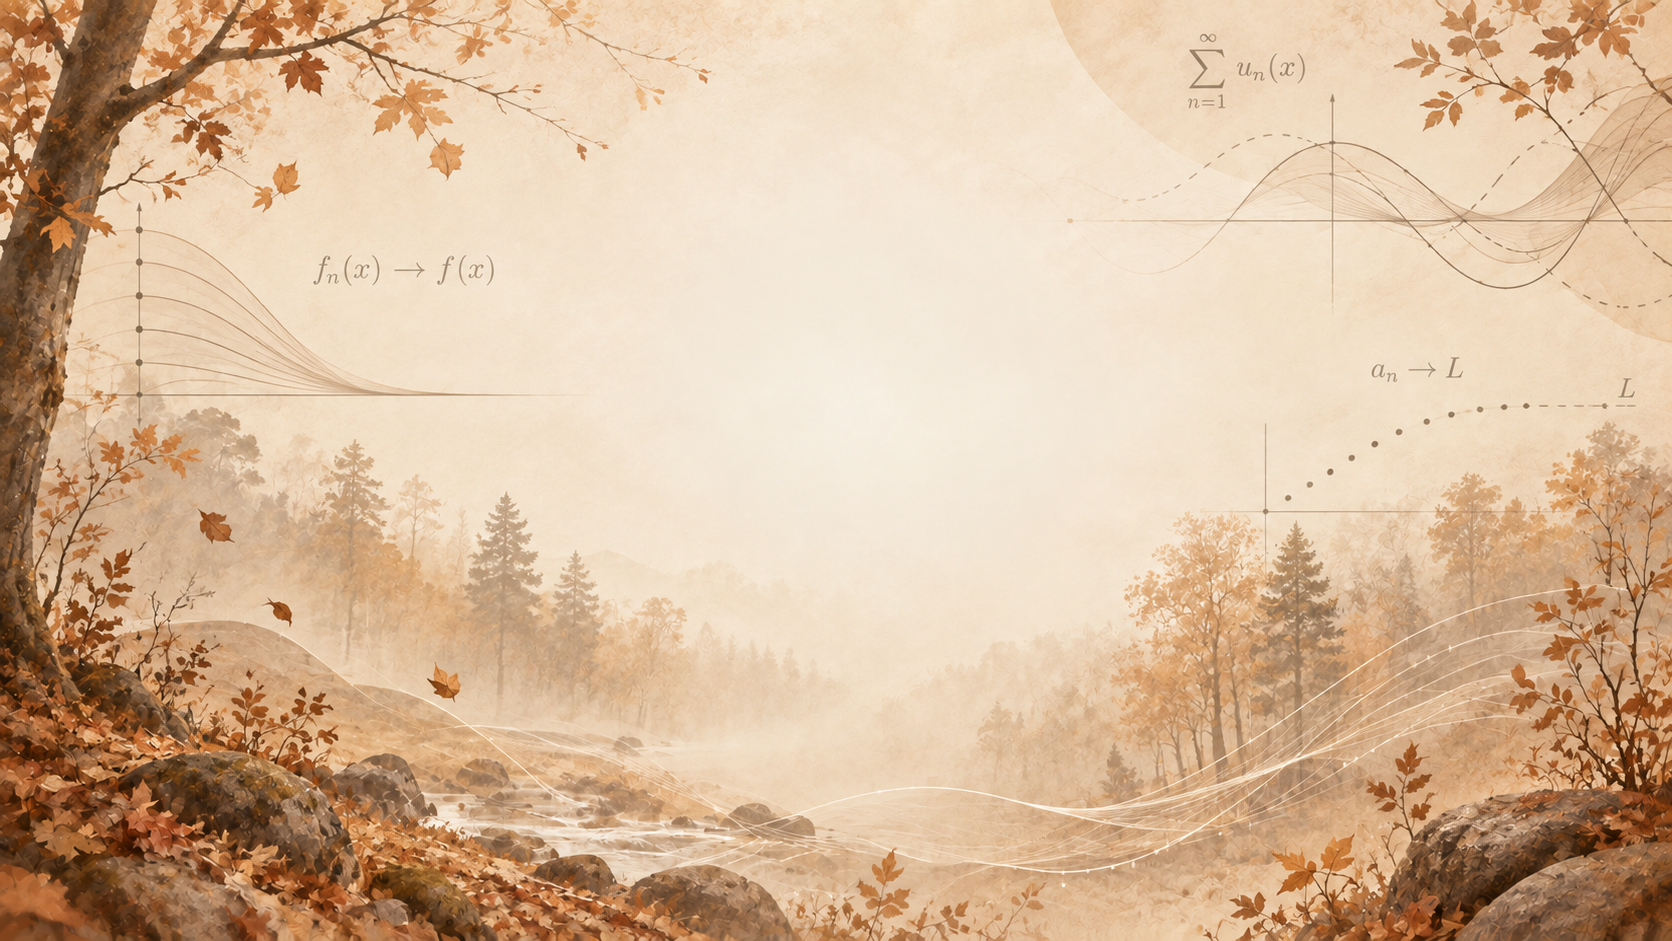
\includegraphics[width=\paperwidth,height=\paperheight,keepaspectratio=false]{chapter_07_bg_01.png}%
}
\begin{frame}[c]{Outline}
  \begin{center}
    \tableofcontents
  \end{center}

  \note{
    Here is the plan. We start with motivation: why limits of
    functions are a new kind of question. Then we give Definition 7.1,
    pointwise convergence of sequences and of series of functions, and
    draw a picture of what it means. Next we state the main problem
    precisely, and we see that it is really a question about
    interchanging two limit processes. The heart of the section is a
    sequence of five examples, 7.2 through 7.6. Example 7.2 is a
    double sequence of numbers where the two iterated limits disagree.
    Example 7.3 is a series of continuous functions with a
    discontinuous sum. Example 7.4 produces a limit function that is
    discontinuous everywhere and not even integrable. Example 7.5
    shows that derivatives need not converge, and Example 7.6 shows
    that integrals need not converge. We close with a summary and a
    look ahead to uniform convergence.
  }
\end{frame}

\section{Motivation}

% --- Build 1/4 ---
\begin{frame}{Why This Section Matters}

  \begin{hlbox}  \begin{itemize}
    \item So far: limits of \alert{numbers}.\\
      Now: limits of \alert{functions} $f_1, f_2, f_3, \dots$ on a set $E$
  \end{itemize}
  \end{hlbox}

\note{
    Let's start with the big picture. Everything we have done so far,
    convergent sequences in Chapter 3, continuity in Chapter 4,
    derivatives in Chapter 5, integrals in Chapter 6, involved limits
    of numbers. Now the objects in the sequence are functions: "f" sub
    1, "f" sub 2, "f" sub 3, and so on, all defined on a common set
    capital "E". We want to make sense of a limit function "f", and
    the natural first idea is to take the limit at each point of
    capital "E" separately. That is the definition we will give in a
    moment. Next, the real question.
  }
\end{frame}

% --- Build 2/4 ---
\begin{frame}{Why This Section Matters}

  \begin{hlbox}  \begin{itemize}
    \item So far: limits of \alert{numbers}.\\
      Now: limits of \alert{functions} $f_1, f_2, f_3, \dots$ on a set $E$
    \item Central question: do \emph{continuity}, \emph{differentiability},
      \emph{integrability} \alert{survive} the limit $f_n \to f$?
  \end{itemize}
  \end{hlbox}

\note{
    The central question is whether the good properties of the
    individual functions are inherited by the limit. If every "f" sub
    "n" is continuous, is "f" continuous? If every "f" sub "n" is
    differentiable, is "f" differentiable, and is the derivative of
    "f" the limit of the derivatives? If every "f" sub "n" is
    integrable, is "f" integrable, and is the integral of "f" the
    limit of the integrals? In calculus one often takes such things
    for granted, differentiating a series term by term or integrating
    under a limit sign. This chapter asks when that is legitimate.
  }
\end{frame}

% --- Build 3/4 ---
\begin{frame}{Why This Section Matters}

  \begin{hlbox}  \begin{itemize}
    \item So far: limits of \alert{numbers}.\\
      Now: limits of \alert{functions} $f_1, f_2, f_3, \dots$ on a set $E$
    \item Central question: do \emph{continuity}, \emph{differentiability},
      \emph{integrability} \alert{survive} the limit $f_n \to f$?
    \item Each of these is a question about \alert{interchanging two limit
      processes}, e.g.\ $\lim_{t \to x}$ and $\lim_{n \to \infty}$
  \end{itemize}
  \end{hlbox}

\note{
    Here is the unifying viewpoint. Continuity is a limit, the
    derivative is a limit, and the integral is a limit too. So asking
    whether continuity survives the passage to "f" is asking whether
    we may swap the limit as "t" goes to "x" with the limit as "n"
    goes to infinity. Asking about derivatives and integrals is asking
    whether we may swap those limits with the limit in "n". Every
    question in this chapter is a question about the order of two
    limit processes.
  }
\end{frame}

% --- Build 4/4 ---
\begin{frame}{Why This Section Matters}

  \begin{hlbox}  \begin{itemize}
    \item So far: limits of \alert{numbers}.\\
      Now: limits of \alert{functions} $f_1, f_2, f_3, \dots$ on a set $E$
    \item Central question: do \emph{continuity}, \emph{differentiability},
      \emph{integrability} \alert{survive} the limit $f_n \to f$?
    \item Each of these is a question about \alert{interchanging two limit
      processes}, e.g.\ $\lim_{t \to x}$ and $\lim_{n \to \infty}$
    \item This section: five examples where the answer is \alert{no}.\\
      Next section: the fix, \alert{uniform convergence}.
  \end{itemize}
  \end{hlbox}

\note{
    And here is the plan for this section. We will see five examples,
    numbered 7.2 through 7.6, in which limits cannot be interchanged:
    the answer to our question is no. These examples are not
    pathological curiosities; they are simple, explicit formulas, and
    they show that pointwise convergence is too weak to carry
    properties over to the limit. In the next section we introduce a
    stronger mode of convergence, uniform convergence, under which the
    order of limit processes does not matter. First, a word about the
    setting.
  }
\end{frame}

\begin{frame}{The Setting for Chapter 7}
  \begin{remblock}{Standing convention}
    All functions are \alert{complex-valued} (real-valued functions included),
    defined on a set $E$.
  \end{remblock}
  \begin{hlbox}

  \vspace{0.6em}
  \begin{itemize}
    \item Most theorems and proofs extend without difficulty to
      \emph{vector-valued} functions, even to maps into general metric spaces
    \item We stay in the simple setting to focus on the real issue:
      \alert{interchanging limit processes}
  \end{itemize}
  \end{hlbox}

\note{
    Before the definitions, a standing convention for the whole
    chapter, shown in the gray box. All functions are complex valued,
    and of course real valued functions are included as a special
    case. As the bullets say, most of the theorems and proofs extend
    without difficulty to vector valued functions, and even to
    mappings into general metric spaces, where the absolute value is
    replaced by the metric. Rudin deliberately stays within the
    simplest framework so that our attention is on the important
    issue, the interchange of limit processes, rather than on
    notation. Now let's define pointwise convergence.
  }
\end{frame}
}

{
\usebackgroundtemplate{%
  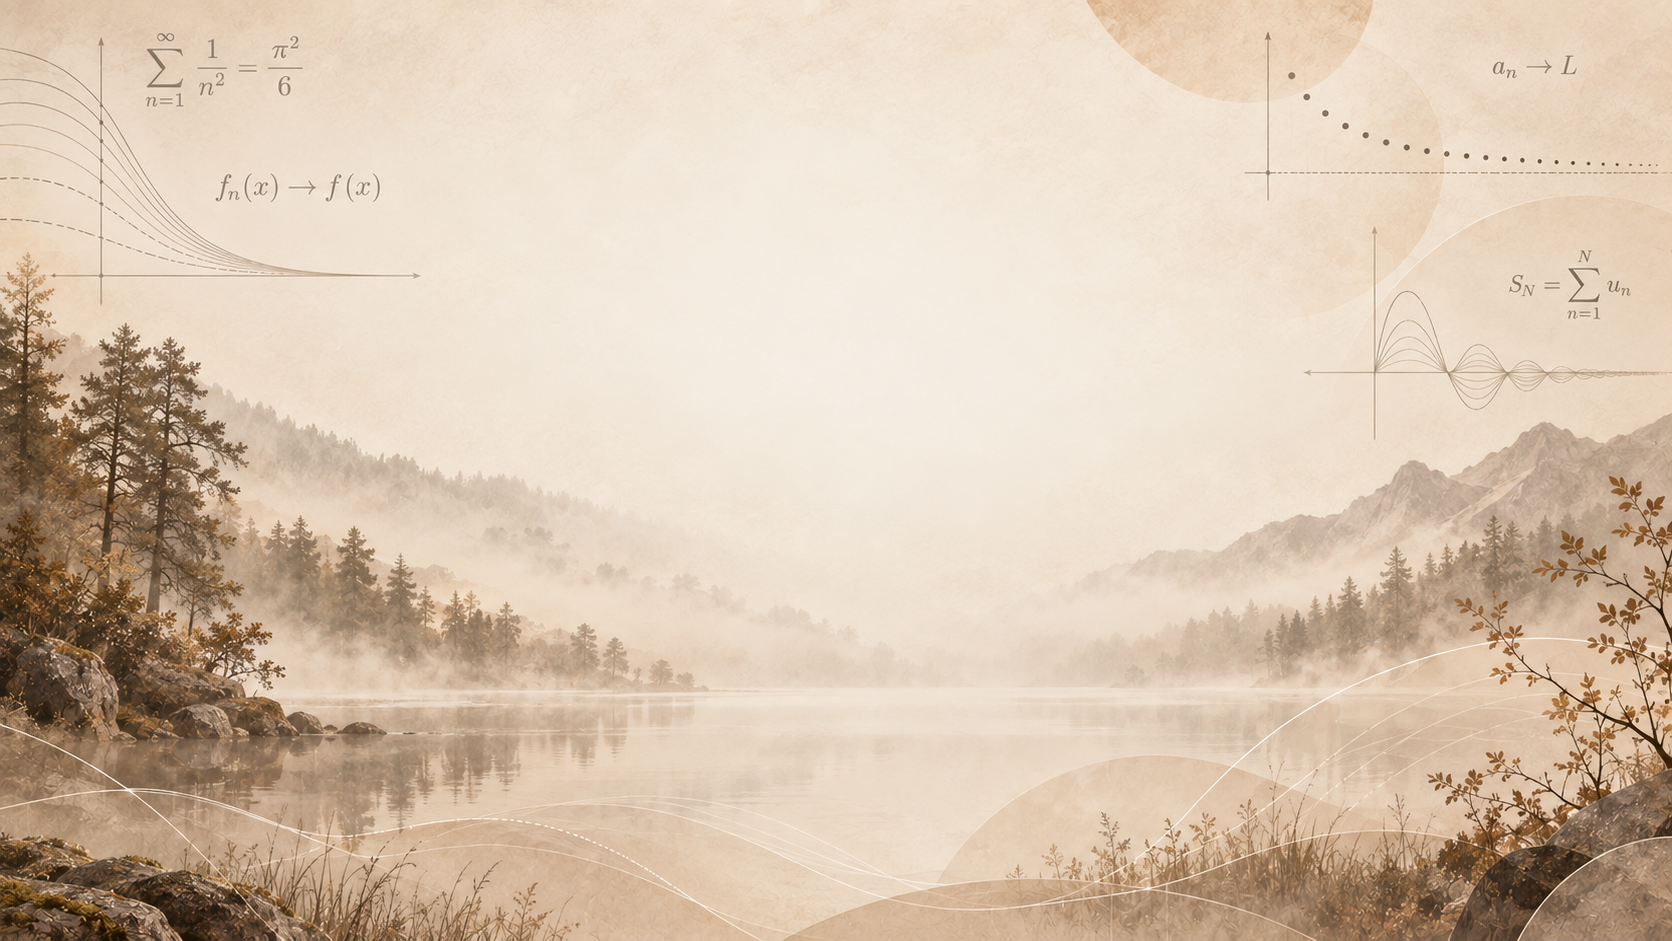
\includegraphics[width=\paperwidth,height=\paperheight,keepaspectratio=false]{chapter_07_bg_02.png}%
}
\section{Pointwise Convergence}

% --- Build 1/2 ---
\begin{frame}{Definition 7.1: Pointwise Convergence}
  \begin{defblock}{Definition 7.1 (sequences)}
    Let $\{f_n\}$, $n = 1, 2, 3, \dots$, be functions on a set $E$ such that the
    sequence of \emph{numbers} $\{f_n(x)\}$ converges for every $x \in E$. Define
    \begin{equation}
      f(x) = \lim_{n \to \infty} f_n(x) \qquad (x \in E). \tag{1}
    \end{equation}
    Then $\{f_n\}$ \alert{converges on $E$}, $f$ is its \alert{limit function},
    and ``$\{f_n\}$ converges to $f$ \alert{pointwise} on $E$.''
  \end{defblock}

  \note{
    Here is Definition 7.1 for sequences. We have functions "f" sub
    "n" on a set capital "E". Fix a point "x" in capital "E" and look
    at the numbers "f" sub 1 of "x", "f" sub 2 of "x", "f" sub 3 of
    "x", and so on. This is an ordinary sequence of numbers. If it
    converges for every "x" in capital "E", we define "f" of "x" to be
    its limit; that is equation 1. Then we say the sequence converges
    on capital "E", and "f" is the limit function. The more
    descriptive phrase, which we will use constantly, is that "f" sub
    "n" converges to "f" pointwise on capital "E": the convergence
    happens one point at a time. Next, the same idea for series.
  }
\end{frame}

% --- Build 2/2 ---
\begin{frame}{Definition 7.1: Pointwise Convergence}
  \begin{defblock}{Definition 7.1 (sequences)}
    Let $\{f_n\}$, $n = 1, 2, 3, \dots$, be functions on a set $E$ such that the
    sequence of \emph{numbers} $\{f_n(x)\}$ converges for every $x \in E$. Define
    \begin{equation}
      f(x) = \lim_{n \to \infty} f_n(x) \qquad (x \in E). \tag{1}
    \end{equation}
    Then $\{f_n\}$ \alert{converges on $E$}, $f$ is its \alert{limit function},
    and ``$\{f_n\}$ converges to $f$ \alert{pointwise} on $E$.''
  \end{defblock}

  \begin{defblock}{Definition 7.1 (series)}
    If $\sum f_n(x)$ converges for every $x \in E$, then the function\\
    $f(x) = \sum_{n=1}^{\infty} f_n(x)$ \ $(x \in E)$ \hfill (2)\\[2pt]
    is called the \alert{sum} of the series $\sum f_n$.
  \end{defblock}

  \note{
    Similarly for series. If for every "x" in capital "E" the
    numerical series, the sum over "n" of "f" sub "n" of "x",
    converges, we define "f" of "x" to be its sum; that is equation 2,
    and "f" is called the sum of the series. Of course a series is
    just the sequence of its partial sums, so equation 2 is equation 1
    applied to the partial sum functions "s" sub capital "N" of "x", the sum
    of the first capital "N" terms. Everything we say about sequences
    of functions therefore applies to series of functions as well.
    Let's look at a picture of pointwise convergence.
  }
\end{frame}

\begin{frame}[c]{Pointwise Convergence: A Picture}
  \begin{center}
  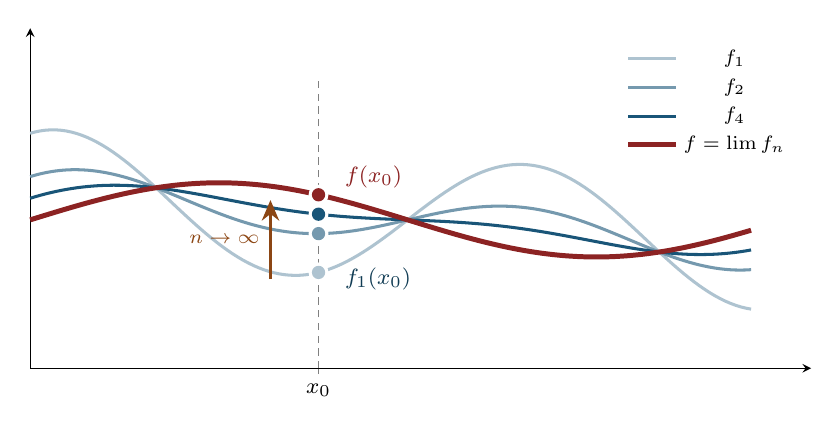
\begin{tikzpicture}
    \begin{axis}[
      width=11.5cm, height=5.9cm,
      axis lines=left,
      xmin=0, xmax=3.25, ymin=0, ymax=2.75,
      xtick={1.2}, xticklabels={$x_0$},
      ytick=\empty,
      tick label style={font=\footnotesize},
      legend style={font=\scriptsize, at={(0.985,0.97)}, anchor=north east,
        draw=none, fill=white, fill opacity=0.8, text opacity=1},
      clip=false,
    ]
      \addplot[defcolor!35, line width=1.1pt, domain=0:3, samples=140]
        {1.2 + 0.3*sin(deg(2*x)) + 0.7*cos(deg(3*x))};
      \addlegendentry{$f_1$}
      \addplot[defcolor!60, line width=1.1pt, domain=0:3, samples=140]
        {1.2 + 0.3*sin(deg(2*x)) + 0.35*cos(deg(3*x))};
      \addlegendentry{$f_2$}
      \addplot[defcolor, line width=1.1pt, domain=0:3, samples=140]
        {1.2 + 0.3*sin(deg(2*x)) + 0.175*cos(deg(3*x))};
      \addlegendentry{$f_4$}
      \addplot[thmcolor, line width=1.8pt, domain=0:3, samples=140]
        {1.2 + 0.3*sin(deg(2*x))};
      \addlegendentry{$f = \lim f_n$}
      \draw[projln, gray] (axis cs:1.2,0) -- (axis cs:1.2,2.35);
      \dotpt{defcolor!35}{(axis cs:1.2,0.775)}
      \dotpt{defcolor!60}{(axis cs:1.2,1.089)}
      \dotpt{defcolor}{(axis cs:1.2,1.246)}
      \dotpt{thmcolor}{(axis cs:1.2,1.403)}
      \node[thmcolor, font=\footnotesize, anchor=west] at (axis cs:1.27,1.55) {$f(x_0)$};
      \node[defcolor!70!black, font=\footnotesize, anchor=west] at (axis cs:1.27,0.72) {$f_1(x_0)$};
      \draw[guide, mAccent] (axis cs:1.0,0.72) -- (axis cs:1.0,1.36)
        node[midway, left, font=\scriptsize] {$n \to \infty$};
    \end{axis}
  \end{tikzpicture}
  \end{center}

  \note{
    Looking at the diagram: the thick red curve is the limit function
    "f". The three blue curves are "f" sub 1, "f" sub 2, and "f" sub
    4, drawn in progressively darker blue; each is a wiggly
    perturbation of "f", and the wiggles shrink as "n" grows. Now
    freeze a point "x" sub 0, marked by the vertical dashed gray line.
    Along that line sit the dots "f" sub 1 of "x" sub 0, "f" sub 2 of
    "x" sub 0, "f" sub 4 of "x" sub 0, climbing toward the red dot "f"
    of "x" sub 0, as the orange arrow indicates. That is all pointwise
    convergence asks: for each fixed "x", the numbers "f" sub "n" of
    "x" converge to "f" of "x". Nothing is said about how the
    different points relate to one another, and that omission is the
    root of every problem in this section.
  }
\end{frame}

% --- Build 1/2 ---
\begin{frame}{Unpacking ``Pointwise''}
  \begin{remblock}{Definition 7.1 in $\varepsilon$--$N$ form}
    $f_n \to f$ pointwise on $E$ means: for every $x \in E$ and every
    $\varepsilon > 0$ there is an integer $N$ such that
    \[
      |f_n(x) - f(x)| < \varepsilon \qquad \text{for all } n \geq N.
    \]
  \end{remblock}
  \begin{hlbox}

  \vspace{0.6em}
  \begin{itemize}
    \item The integer $N$ is chosen \alert{after} $x$: $N = N(\varepsilon, x)$
  \end{itemize}
  \end{hlbox}

\note{
    Let's unpack the definition in epsilon and capital "N" language,
    as in the gray box. Pointwise convergence means: for every point
    "x" in capital "E" and every epsilon greater than zero, there is
    an integer capital "N" such that the distance between "f" sub "n"
    of "x" and "f" of "x" is less than epsilon whenever "n" is at
    least capital "N". The crucial point is the order of the
    quantifiers. The point "x" is fixed first, and capital "N" is
    chosen afterward, so capital "N" depends on both epsilon and "x".
    Different points may need very different thresholds.
  }
\end{frame}

% --- Build 2/2 ---
\begin{frame}{Unpacking ``Pointwise''}
  \begin{remblock}{Definition 7.1 in $\varepsilon$--$N$ form}
    $f_n \to f$ pointwise on $E$ means: for every $x \in E$ and every
    $\varepsilon > 0$ there is an integer $N$ such that
    \[
      |f_n(x) - f(x)| < \varepsilon \qquad \text{for all } n \geq N.
    \]
  \end{remblock}
  \begin{hlbox}

  \vspace{0.6em}
  \begin{itemize}
    \item The integer $N$ is chosen \alert{after} $x$: $N = N(\varepsilon, x)$
    \item At some points convergence may be fast, at others \emph{slow}
    \item This is exactly the loophole the examples will exploit
  \end{itemize}
  \end{hlbox}

\note{
    Because the threshold may change from point to point, the
    convergence can be fast at some points while at nearby points it
    is arbitrarily slow, with no single capital "N" that serves all of
    capital "E" at once. As the last bullet says, this is precisely
    the loophole that the upcoming examples exploit: they hide the bad
    behavior in the region where convergence is slow. Closing this
    loophole, by demanding one capital "N" for all points, will be
    the idea behind uniform convergence in the next section. Now let's
    state the main problem.
  }
\end{frame}
}

{
\usebackgroundtemplate{%
  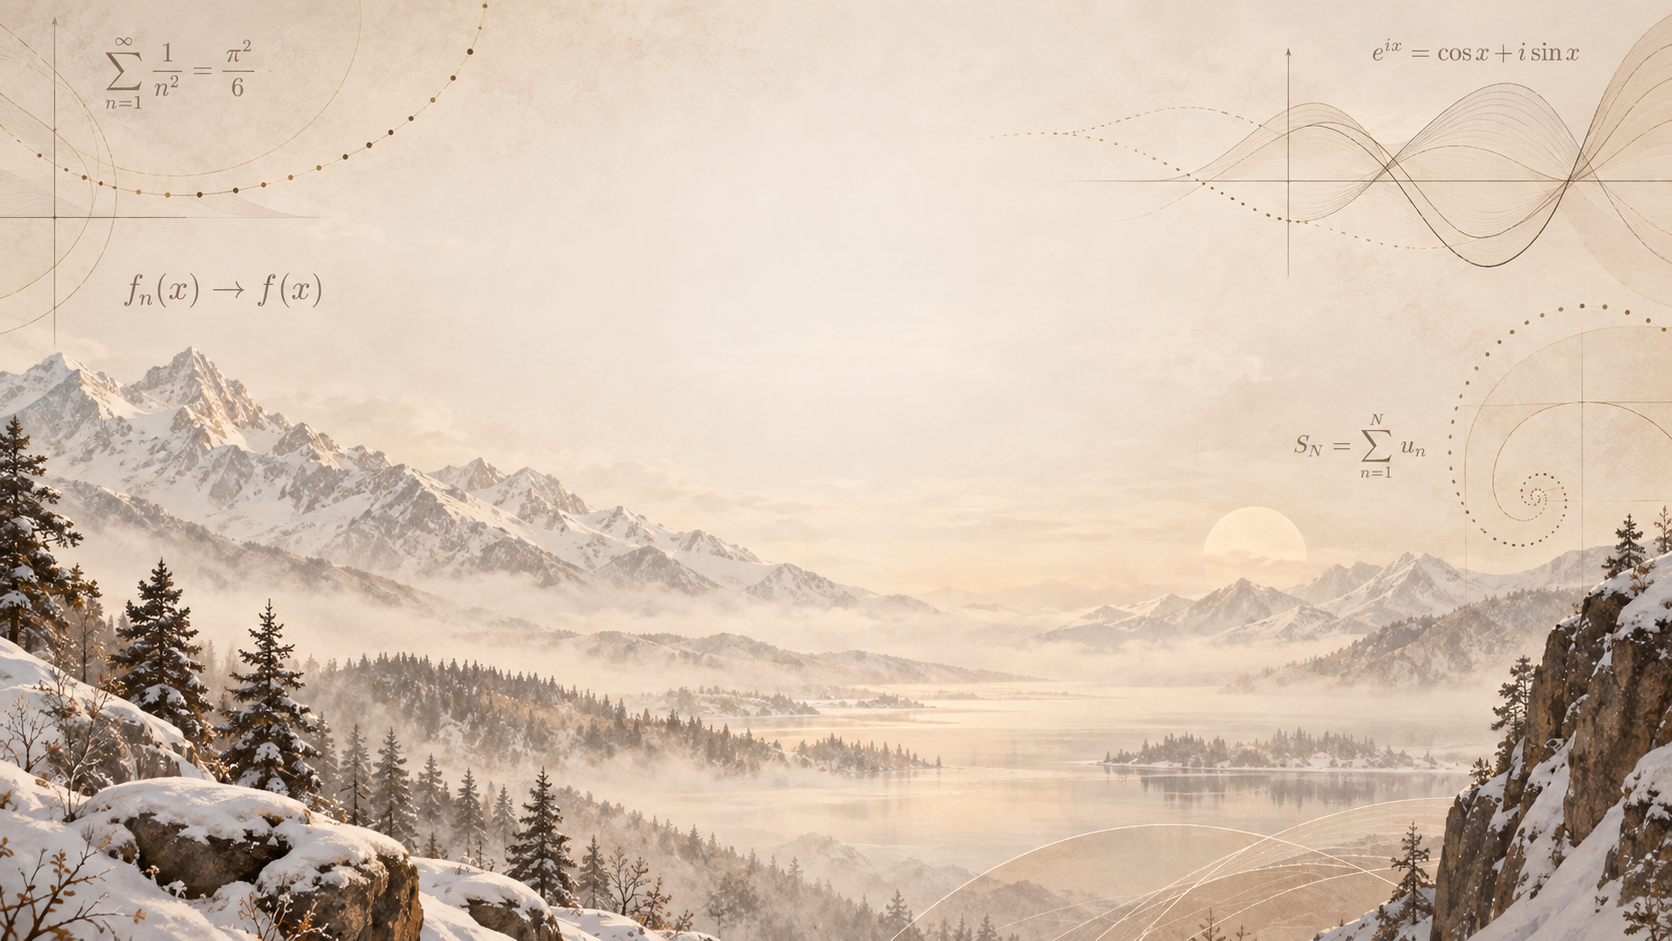
\includegraphics[width=\paperwidth,height=\paperheight,keepaspectratio=false]{chapter_07_bg_03.png}%
}
\section{The Main Problem}

% --- Build 1/3 ---
\begin{frame}{The Main Problem}

  \begin{hlbox}  \textbf{Are important properties of $f_n$ preserved under the limit
  operations (1) and (2)?}

  \vspace{0.6em}
  \begin{itemize}
    \item If each $f_n$ is \alert{continuous}, is $f$ continuous?
  \end{itemize}
  \end{hlbox}

\note{
    The main problem, stated in bold at the top of the slide, is
    whether important properties of the functions "f" sub "n" are
    preserved under the limit operations in equations 1 and 2. The
    first instance is continuity. If each "f" sub "n" is continuous,
    is the limit function "f" continuous? Intuitively, "f" is
    approximated by continuous functions, so one might hope so. We
    will see in Example 7.3 that the hope is misplaced. Next,
    derivatives.
  }
\end{frame}

% --- Build 2/3 ---
\begin{frame}{The Main Problem}

  \begin{hlbox}  \textbf{Are important properties of $f_n$ preserved under the limit
  operations (1) and (2)?}

  \vspace{0.6em}
  \begin{itemize}
    \item If each $f_n$ is \alert{continuous}, is $f$ continuous?
    \item If each $f_n$ is \alert{differentiable}, is $f$ differentiable?
      How are $f_n'$ and $f'$ related? Is $f' = \lim f_n'$?
  \end{itemize}
  \end{hlbox}

\note{
    The second instance is differentiability. If each "f" sub "n" is
    differentiable, is "f" differentiable? And even if it is, what is
    the relation between the derivatives "f" sub "n" prime and the
    derivative "f" prime? The natural guess is that "f" prime is the
    limit of the "f" sub "n" prime, which is what one does when
    differentiating a power series term by term. Example 7.5 will
    show that in general this fails badly. Next, integrals.
  }
\end{frame}

% --- Build 3/3 ---
\begin{frame}{The Main Problem}

  \begin{hlbox}  \textbf{Are important properties of $f_n$ preserved under the limit
  operations (1) and (2)?}

  \vspace{0.6em}
  \begin{itemize}
    \item If each $f_n$ is \alert{continuous}, is $f$ continuous?
    \item If each $f_n$ is \alert{differentiable}, is $f$ differentiable?
      How are $f_n'$ and $f'$ related? Is $f' = \lim f_n'$?
    \item If each $f_n$ is \alert{integrable}, is $f$ integrable?
      Is $\int f = \lim \int f_n$?
  \end{itemize}
  \end{hlbox}

\note{
    The third instance is integrability. If each "f" sub "n" is
    Riemann integrable, is "f" integrable? And is the integral of "f"
    the limit of the integrals of the "f" sub "n"? Example 7.4 will
    give a limit function that is not integrable at all, and Example
    7.6 will give integrable functions whose integrals do not converge
    to the integral of the limit. To see what all three questions have
    in common, let's look closely at the first one.
  }
\end{frame}

% --- Build 1/2 ---
\begin{frame}{Continuity as an Interchange of Limits}

  \begin{hlbox}  $f$ is continuous at a limit point $x$ of $E$ means
  \[
    \lim_{t \to x} f(t) = f(x).
  \]

  \vspace{0.3em}
  So ``\emph{is the limit of continuous functions continuous?}''
  is the same as asking whether
  \begin{equation}
    \lim_{t \to x}\, \lim_{n \to \infty} f_n(t)
    \;=\;
    \lim_{n \to \infty}\, \lim_{t \to x} f_n(t), \tag{3}
  \end{equation}
  i.e.\ whether the \alert{order of the two limit processes is immaterial}.
  \end{hlbox}

\note{
    Continuity is itself a limit statement. To say that "f" is
    continuous at a limit point "x" of capital "E" means that the
    limit of "f" of "t" as "t" goes to "x" equals "f" of "x". Now
    substitute the definition of "f" as a limit of the "f" sub "n".
    The left side becomes the limit as "t" goes to "x" of the limit as
    "n" goes to infinity of "f" sub "n" of "t". On the right, "f" of
    "x" is the limit as "n" goes to infinity of "f" sub "n" of "x",
    and since each "f" sub "n" is continuous, "f" sub "n" of "x" is
    the limit as "t" goes to "x" of "f" sub "n" of "t". That gives
    equation 3. So the question about continuity is exactly the
    question whether the two limit processes may be interchanged.
  }
\end{frame}

% --- Build 2/2 ---
\begin{frame}{Continuity as an Interchange of Limits}

  \begin{hlbox}  $f$ is continuous at a limit point $x$ of $E$ means
  \[
    \lim_{t \to x} f(t) = f(x).
  \]

  \vspace{0.3em}
  So ``\emph{is the limit of continuous functions continuous?}''
  is the same as asking whether
  \begin{equation}
    \lim_{t \to x}\, \lim_{n \to \infty} f_n(t)
    \;=\;
    \lim_{n \to \infty}\, \lim_{t \to x} f_n(t), \tag{3}
  \end{equation}
  i.e.\ whether the \alert{order of the two limit processes is immaterial}.

  \vspace{0.3em}
  \begin{itemize}
    \item Left side of (3): first $n \to \infty$, then $t \to x$
    \item Right side of (3): first $t \to x$, then $n \to \infty$
  \end{itemize}
  \end{hlbox}

\note{
    Read equation 3 from the inside out. On the left side we first
    let "n" go to infinity, producing the limit function, and only
    then let "t" go to "x". On the right side we first let "t" go to
    "x" inside each "f" sub "n", and only then let "n" go to infinity.
    The two sides use the same ingredients in the opposite order, and
    equation 3 asks whether the order is immaterial. Let's draw this.
  }
\end{frame}

\begin{frame}[c]{Two Routes from $f_n(t)$ to $f(x)$}
  \begin{center}
  \begin{hlbox}[hbox]
  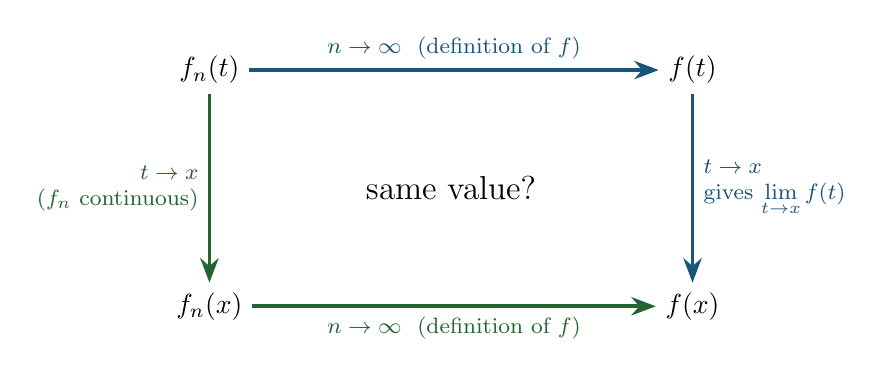
\begin{tikzpicture}[>=Stealth, node distance=2.4cm and 5.2cm,
      every node/.style={font=\normalsize}]
    \node (a) {$f_n(t)$};
    \node (b) [right=of a] {$f(t)$};
    \node (c) [below=of a] {$f_n(x)$};
    \node (d) [below=of b] {$f(x)$};
    \node (q) at ($(a)!0.5!(d)$) {\alert{\large same value?}};
    \draw[->, line width=1.3pt, defcolor] (a) -- node[above, font=\footnotesize]
      {$n \to \infty$ \ (definition of $f$)} (b);
    \draw[->, line width=1.3pt, defcolor] (b) -- node[right, font=\footnotesize, align=left]
      {$t \to x$\\ gives $\lim\limits_{t \to x} f(t)$} (d);
    \draw[->, line width=1.3pt, proofcolor] (a) -- node[left, font=\footnotesize, align=right]
      {$t \to x$\\ ($f_n$ continuous)} (c);
    \draw[->, line width=1.3pt, proofcolor] (c) -- node[below, font=\footnotesize]
      {$n \to \infty$ \ (definition of $f$)} (d);
  \end{tikzpicture}
  \end{hlbox}
  \end{center}

  \vspace{0.2em}
  \begin{center}
    \hl{\textcolor{defcolor}{\textbf{Blue route}} $=$ left side of (3)
    \qquad
    \textcolor{proofcolor}{\textbf{Green route}} $=$ right side of (3)}
  \end{center}

  \note{
    The diagram shows the two routes. We start in the top left corner
    with "f" sub "n" of "t". The blue route goes first to the right:
    let "n" go to infinity, which by definition gives "f" of "t"; then
    down: let "t" go to "x", which gives the limit of "f" of "t" as
    "t" approaches "x". That is the left side of equation 3. The green
    route goes first down: let "t" go to "x", which by continuity of
    "f" sub "n" gives "f" sub "n" of "x"; then to the right: let "n"
    go to infinity, which by definition gives "f" of "x". That is the
    right side of equation 3. The question in the middle of the
    square, highlighted in orange, is whether both routes arrive at
    the same value. When they do, "f" is continuous at "x". Now let's
    preview the examples that show they need not.
  }
\end{frame}

\begin{frame}{Plan: What Can Go Wrong}

  \begin{hlbox}  \textbf{Limit processes cannot in general be interchanged.}
  Five examples:

  \vspace{0.2em}
  \begin{center}
  \renewcommand{\arraystretch}{1.15}\small
  \begin{tabular}{@{}lll@{}}
    \textbf{Example} & \textbf{Object} & \textbf{Failure} \\ \hline
    7.2 & double sequence $s_{m,n}$ & $\lim_n \lim_m \neq \lim_m \lim_n$ \\
    7.3 & series of continuous $f_n$ & sum $f$ is \alert{discontinuous} \\
    7.4 & iterated limit of $\cos^{2n}$ & $f$ nowhere continuous, \alert{not integrable} \\
    7.5 & $f_n = \sin(nx)/\sqrt{n}$ & $f_n' \not\to f'$ \\
    7.6 & $f_n = n^2 x (1-x^2)^n$ & $\int f_n \not\to \int f$ \\
  \end{tabular}
  \end{center}

  \vspace{0.2em}
  \textbf{Afterward}: conditions under which the order
  \emph{is} immaterial.
  \end{hlbox}

\note{
    Here is the plan for the rest of the section, in the table. Rudin
    shows by means of several examples that limit processes cannot in
    general be interchanged without affecting the result. Example 7.2
    is the simplest: a double sequence of numbers "s" with indices "m" and
    "n", where taking the limits in the two possible orders gives two
    different answers. Example 7.3 is a series of continuous functions
    whose sum is discontinuous. Example 7.4 produces, by two limits in
    a row, a function that is discontinuous at every point and not
    Riemann integrable. Example 7.5 shows that derivatives of the "f"
    sub "n" need not converge to the derivative of "f". Example 7.6
    shows that the integrals of the "f" sub "n" need not converge to
    the integral of "f". After these warnings, the later sections of
    the chapter prove that under suitable conditions the order of
    limit operations is immaterial. Let's start with Example 7.2.
  }
\end{frame}
}

{
\usebackgroundtemplate{%
  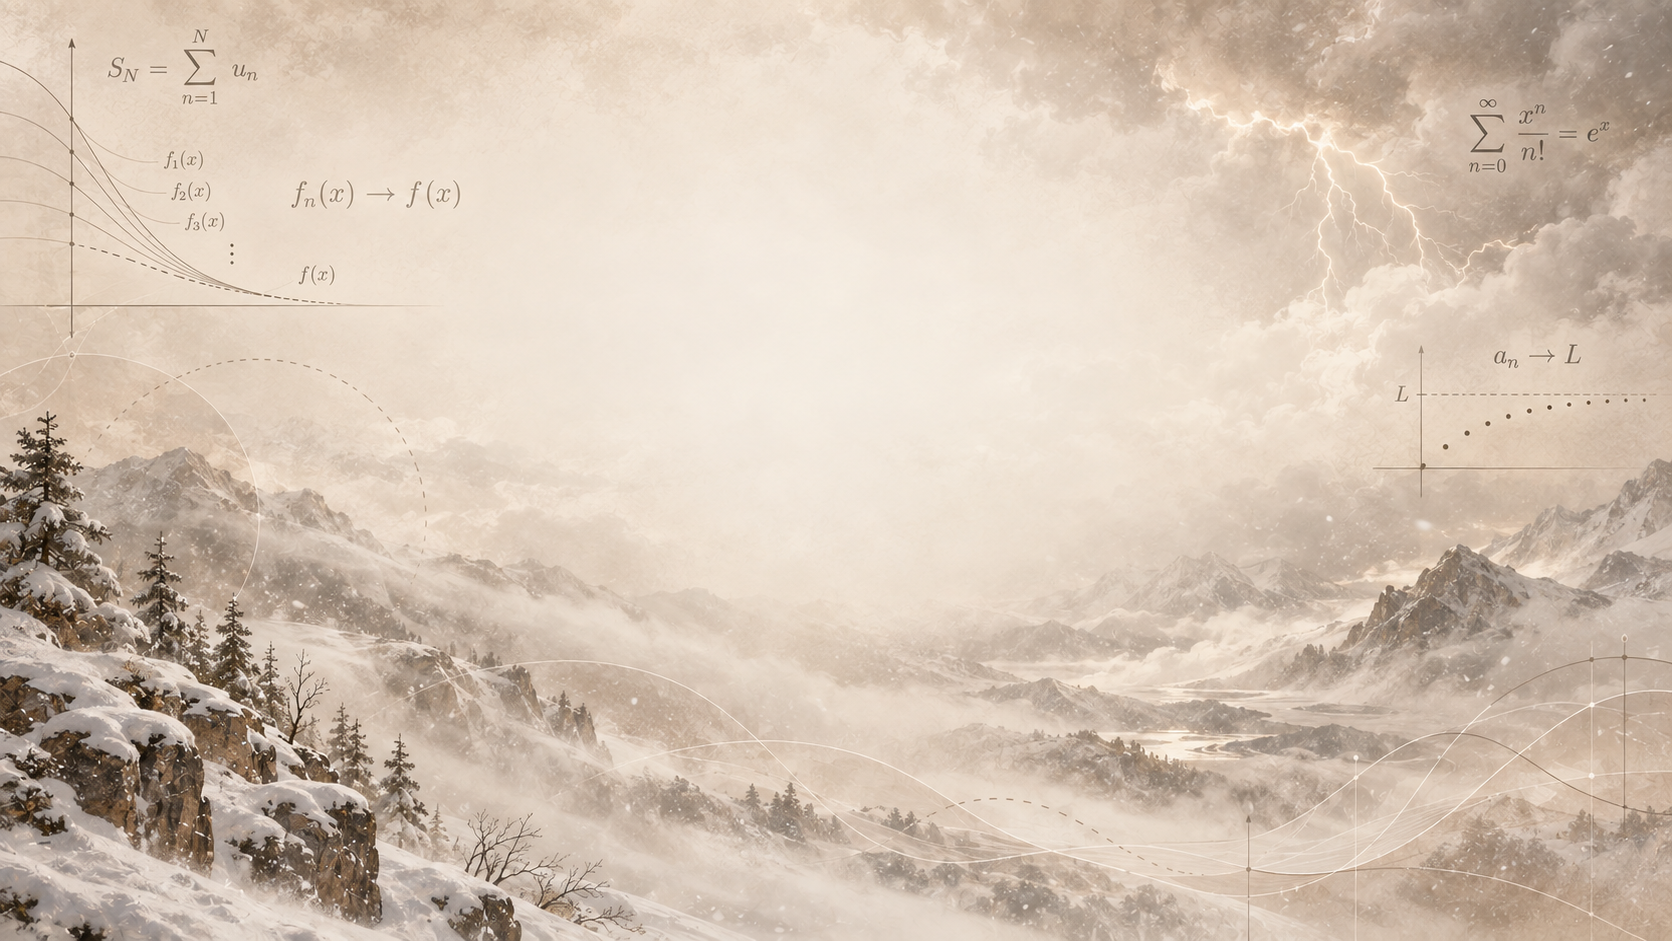
\includegraphics[width=\paperwidth,height=\paperheight,keepaspectratio=false]{chapter_07_bg_04.png}%
}
\section{Example 7.2: A Double Sequence}

% --- Build 1/4 ---
\begin{frame}{Example 7.2: A Double Sequence}
  \begin{exblock}{Example 7.2}
    For $m = 1, 2, 3, \dots$ and $n = 1, 2, 3, \dots$, let \quad
    $s_{m,n} = \dfrac{m}{m + n}$.
  \end{exblock}

  \note{
    Our first example, and the simplest one, concerns a double
    sequence: a number "s" with two indices "m" and "n", one for every pair of
    positive integers "m" and "n". The formula is "m" divided by "m"
    plus "n". Notice that "s" is always strictly between 0 and 1, and
    it is symmetric in a certain sense: swapping "m" and "n" replaces
    "s" by 1 minus "s". There are two natural ways to take a double
    limit: first "m" to infinity and then "n", or the other way
    around. Let's compute both.
  }
\end{frame}

% --- Build 2/4 ---
\begin{frame}{Example 7.2: A Double Sequence}
  \begin{exblock}{Example 7.2}
    For $m = 1, 2, 3, \dots$ and $n = 1, 2, 3, \dots$, let \quad
    $s_{m,n} = \dfrac{m}{m + n}$.
  \end{exblock}
  \begin{hlbox}

  \textbf{Two orders of taking the double limit:}
  \begin{align}
    n \text{ fixed, } m \to \infty \text{ first:}\quad
    & \lim_{m \to \infty} s_{m,n} = 1
    \;\Longrightarrow\; \lim_{n \to \infty}\, \lim_{m \to \infty} s_{m,n} = 1 \tag{4}
  \end{align}
  \end{hlbox}

\note{
    First let "m" go to infinity with "n" held fixed. Then "m" divided
    by "m" plus "n" tends to 1, because the fixed "n" in the
    denominator becomes negligible compared with "m". This is true for
    every fixed "n", so the inner limit is the constant 1, and the
    outer limit as "n" goes to infinity is also 1. That is equation 4.
    Now the other order.
  }
\end{frame}

% --- Build 3/4 ---
\begin{frame}{Example 7.2: A Double Sequence}
  \begin{exblock}{Example 7.2}
    For $m = 1, 2, 3, \dots$ and $n = 1, 2, 3, \dots$, let \quad
    $s_{m,n} = \dfrac{m}{m + n}$.
  \end{exblock}
  \begin{hlbox}

  \textbf{Two orders of taking the double limit:}
  \begin{align}
    n \text{ fixed, } m \to \infty \text{ first:}\quad
    & \lim_{m \to \infty} s_{m,n} = 1
    \;\Longrightarrow\; \lim_{n \to \infty}\, \lim_{m \to \infty} s_{m,n} = 1 \tag{4} \\
    m \text{ fixed, } n \to \infty \text{ first:}\quad
    & \lim_{n \to \infty} s_{m,n} = 0
    \;\Longrightarrow\; \lim_{m \to \infty}\, \lim_{n \to \infty} s_{m,n} = 0 \tag{5}
  \end{align}
  \end{hlbox}

\note{
    Now let "n" go to infinity with "m" held fixed. This time the
    numerator "m" stays put while the denominator "m" plus "n" grows
    without bound, so the quotient tends to 0. Again this holds for
    every fixed "m", so the inner limit is the constant 0 and the
    outer limit as "m" goes to infinity is 0 as well. That is
    equation 5. Compare the two results.
  }
\end{frame}

% --- Build 4/4 ---
\begin{frame}{Example 7.2: A Double Sequence}
  \begin{exblock}{Example 7.2}
    For $m = 1, 2, 3, \dots$ and $n = 1, 2, 3, \dots$, let \quad
    $s_{m,n} = \dfrac{m}{m + n}$.
  \end{exblock}
  \begin{hlbox}

  \textbf{Two orders of taking the double limit:}
  \begin{align}
    n \text{ fixed, } m \to \infty \text{ first:}\quad
    & \lim_{m \to \infty} s_{m,n} = 1
    \;\Longrightarrow\; \lim_{n \to \infty}\, \lim_{m \to \infty} s_{m,n} = 1 \tag{4} \\
    m \text{ fixed, } n \to \infty \text{ first:}\quad
    & \lim_{n \to \infty} s_{m,n} = 0
    \;\Longrightarrow\; \lim_{m \to \infty}\, \lim_{n \to \infty} s_{m,n} = 0 \tag{5}
  \end{align}

  \begin{center}
    $\boxed{1 \neq 0}$ \quad \alert{The order of the two limits matters.}
  \end{center}
  \end{hlbox}

\note{
    Equation 4 gives 1 and equation 5 gives 0. The same double
    sequence, the same two limit operations, and yet the two iterated
    limits are different. This is the whole phenomenon in its purest
    form: the order in which limit processes are carried out can
    change the answer. Every later example is a version of this one,
    dressed up with functions. Let's look at a table of values to see
    why.
  }
\end{frame}

\begin{frame}[c]{Example 7.2: The Table of Values}
  \begin{center}
  \begin{hlbox}[hbox]
  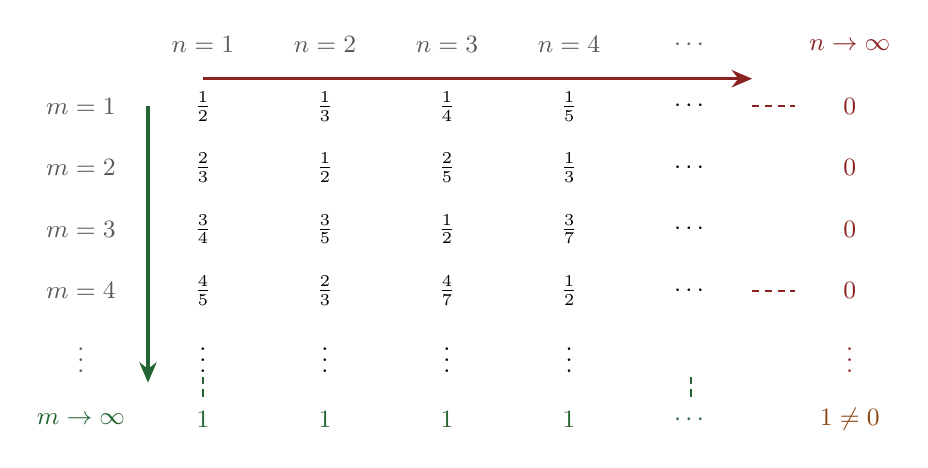
\begin{tikzpicture}[x=1.55cm, y=0.78cm, font=\small]
    % headers
    \foreach \j/\lab in {1/{n=1},2/{n=2},3/{n=3},4/{n=4}}
      \node[remcolor] at (\j,0) {$\lab$};
    \node[remcolor] at (5,0) {$\cdots$};
    \node[thmcolor] at (6.3,0) {$n \to \infty$};
    \foreach \i/\lab in {1/{m=1},2/{m=2},3/{m=3},4/{m=4}}
      \node[remcolor] at (0,-\i) {$\lab$};
    \node[remcolor] at (0,-5) {$\vdots$};
    \node[proofcolor] at (0,-6.1) {$m \to \infty$};
    % values s_{m,n} = m/(m+n)
    \node at (1,-1) {$\tfrac12$}; \node at (2,-1) {$\tfrac13$}; \node at (3,-1) {$\tfrac14$}; \node at (4,-1) {$\tfrac15$};
    \node at (1,-2) {$\tfrac23$}; \node at (2,-2) {$\tfrac12$}; \node at (3,-2) {$\tfrac25$}; \node at (4,-2) {$\tfrac13$};
    \node at (1,-3) {$\tfrac34$}; \node at (2,-3) {$\tfrac35$}; \node at (3,-3) {$\tfrac12$}; \node at (4,-3) {$\tfrac37$};
    \node at (1,-4) {$\tfrac45$}; \node at (2,-4) {$\tfrac23$}; \node at (3,-4) {$\tfrac47$}; \node at (4,-4) {$\tfrac12$};
    \foreach \j in {1,...,4} \node at (\j,-5) {$\vdots$};
    \foreach \i in {1,...,4} \node at (5,-\i) {$\cdots$};
    % row limits (fixed m, n -> infinity): 0
    \foreach \i in {1,...,4} \node[thmcolor] at (6.3,-\i) {$0$};
    \node[thmcolor] at (6.3,-5) {$\vdots$};
    % column limits (fixed n, m -> infinity): 1
    \foreach \j in {1,...,4} \node[proofcolor] at (\j,-6.1) {$1$};
    \node[proofcolor] at (5,-6.1) {$\cdots$};
    % corner
    \node[mAccent, font=\small\bfseries] at (6.3,-6.1) {$1 \neq 0$};
    % arrows
    \draw[guide, thmcolor] (1.0,-0.55) -- (5.5,-0.55);
    \draw[guide, proofcolor] (0.55,-1) -- (0.55,-5.5);
    \draw[projln, proofcolor] (1,-5.4) -- (1,-5.75) (5,-5.4) -- (5,-5.75);
    \draw[projln, thmcolor] (5.5,-1) -- (5.85,-1) (5.5,-4) -- (5.85,-4);
  \end{tikzpicture}
  \end{hlbox}
  \end{center}

  \note{
    The table lists the values of "s" with "m" indexing the rows
    and "n" indexing the columns. Look along the first row, where "m"
    equals 1: one half, one third, one fourth, one fifth, decreasing
    toward 0. Every row does the same, so the red column on the right,
    labeled row limits, is all zeros; these are the limits as "n" goes
    to infinity with "m" fixed, and their limit in "m" is 0, which is
    equation 5. Now look down the first column, where "n" equals 1:
    one half, two thirds, three fourths, four fifths, increasing toward
    1. Every column does the same, so the green row at the bottom,
    labeled column limits, is all ones; their limit in "n" is 1, which
    is equation 4. The corner where the two directions meet, marked in
    orange, is where the disagreement lives. Notice also the diagonal
    of one halves: along the diagonal "m" equals "n" the sequence sits
    at one half, neither 0 nor 1. The double sequence has no single
    limit as "m" and "n" go to infinity together. Now to functions.
  }
\end{frame}
}

{
\usebackgroundtemplate{%
  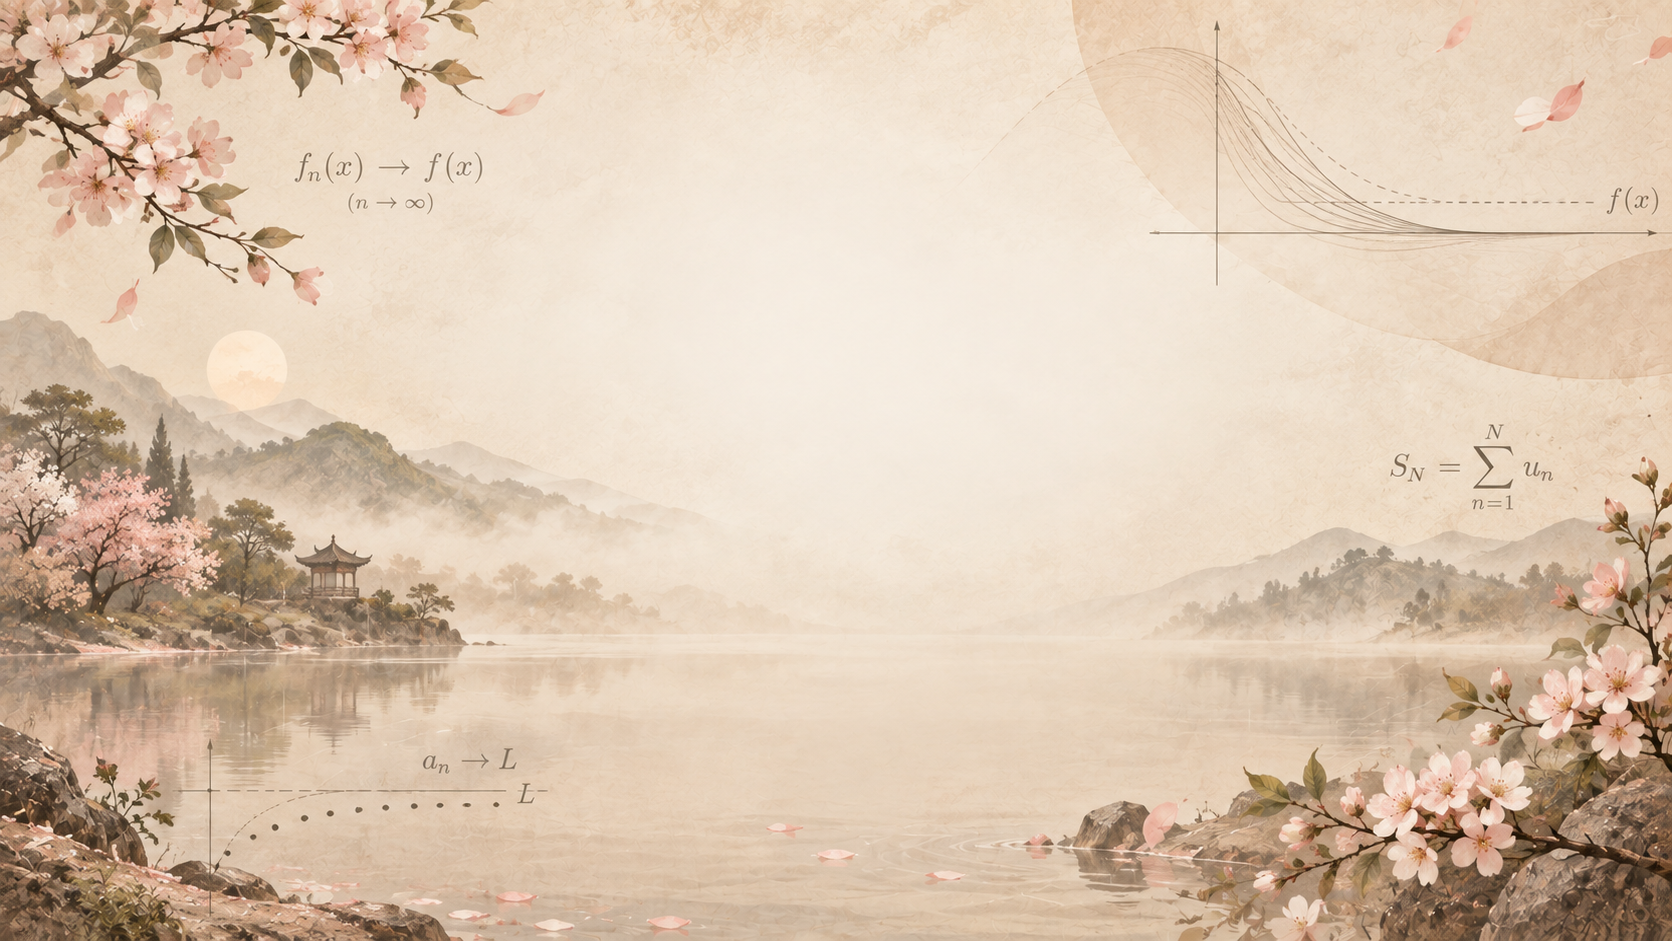
\includegraphics[width=\paperwidth,height=\paperheight,keepaspectratio=false]{chapter_07_bg_05.png}%
}
\section{Example 7.3: A Discontinuous Sum}

% --- Build 1/4 ---
\begin{frame}{Example 7.3: A Series of Continuous Functions}
  \begin{exblock}{Example 7.3}
    For real $x$ and $n = 0, 1, 2, \dots$ (each $f_n$ is \alert{continuous}), let
    \begin{equation}
      f_n(x) = \frac{x^2}{(1 + x^2)^n}, \qquad
      f(x) = \sum_{n=0}^{\infty} f_n(x) = \sum_{n=0}^{\infty} \frac{x^2}{(1 + x^2)^n}. \tag{6}
    \end{equation}
  \end{exblock}


  \note{
    Example 7.3 is a series of functions. The terms are "f" sub "n" of
    "x" equals "x" squared divided by 1 plus "x" squared to the power
    "n", for real "x" and "n" starting at 0. Each term is a quotient
    of polynomials whose denominator never vanishes, so each "f" sub
    "n" is continuous on the whole real line. We consider the series
    in equation 6 and ask what its sum "f" looks like. We treat the
    point "x" equals 0 and the points "x" not equal to 0 separately.
  }
\end{frame}

% --- Build 2/4 ---
\begin{frame}{Example 7.3: A Series of Continuous Functions}
  \begin{exblock}{Example 7.3}
    For real $x$ and $n = 0, 1, 2, \dots$ (each $f_n$ is \alert{continuous}), let
    \begin{equation}
      f_n(x) = \frac{x^2}{(1 + x^2)^n}, \qquad
      f(x) = \sum_{n=0}^{\infty} f_n(x) = \sum_{n=0}^{\infty} \frac{x^2}{(1 + x^2)^n}. \tag{6}
    \end{equation}
  \end{exblock}
  \begin{hlbox}

  \textbf{At $x = 0$:} $f_n(0) = 0$ for every $n$, hence $f(0) = 0$.
  \end{hlbox}

\note{
    At "x" equals 0 the numerator "x" squared is 0, so every term "f"
    sub "n" of 0 vanishes, and the sum of a series of zeros is 0. So
    "f" of 0 equals 0. Now the interesting case, "x" different from 0.
  }
\end{frame}

% --- Build 3/4 ---
\begin{frame}{Example 7.3: A Series of Continuous Functions}
  \begin{exblock}{Example 7.3}
    For real $x$ and $n = 0, 1, 2, \dots$ (each $f_n$ is \alert{continuous}), let
    \begin{equation}
      f_n(x) = \frac{x^2}{(1 + x^2)^n}, \qquad
      f(x) = \sum_{n=0}^{\infty} f_n(x) = \sum_{n=0}^{\infty} \frac{x^2}{(1 + x^2)^n}. \tag{6}
    \end{equation}
  \end{exblock}
  \begin{hlbox}

  \textbf{At $x = 0$:} $f_n(0) = 0$ for every $n$, hence $f(0) = 0$.

  \textbf{At $x \neq 0$:} geometric series with ratio
  $r = \frac{1}{1 + x^2} \in (0, 1)$; by Theorem 3.26,
  \[
    f(x) = x^2 \sum_{n=0}^{\infty} r^n
    = \frac{x^2}{1 - r}
    = \frac{x^2}{\,x^2/(1 + x^2)\,}
    = 1 + x^2.
  \]
  \end{hlbox}

\note{
    For "x" different from 0, pull the factor "x" squared out of the
    sum. What remains is a geometric series with ratio "r" equal to 1
    over 1 plus "x" squared, and since "x" squared is positive, "r"
    lies strictly between 0 and 1. Recall Theorem 3.26: for "r"
    between 0 and 1, the sum of "r" to the "n" from "n" equals 0 to
    infinity is 1 over 1 minus "r". Here 1 minus "r" is "x" squared
    over 1 plus "x" squared, so its reciprocal is 1 plus "x" squared
    over "x" squared. Multiplying by the "x" squared we pulled out,
    the "x" squared cancels and we get "f" of "x" equals 1 plus "x"
    squared, as the chain of equalities on the slide shows. Let's put
    the two cases together.
  }
\end{frame}

% --- Build 4/4 ---
\begin{frame}{Example 7.3: A Series of Continuous Functions}
  \begin{exblock}{Example 7.3}
    For real $x$ and $n = 0, 1, 2, \dots$ (each $f_n$ is \alert{continuous}), let
    \begin{equation}
      f_n(x) = \frac{x^2}{(1 + x^2)^n}, \qquad
      f(x) = \sum_{n=0}^{\infty} f_n(x) = \sum_{n=0}^{\infty} \frac{x^2}{(1 + x^2)^n}. \tag{6}
    \end{equation}
  \end{exblock}
  \begin{hlbox}

  Combining the two cases ($x = 0$; $x \neq 0$ via the geometric series):
  \begin{equation}
    f(x) = \begin{cases} 0 & (x = 0), \\ 1 + x^2 & (x \neq 0). \end{cases} \tag{7}
  \end{equation}

  \begin{center}
    \alert{A convergent series of continuous functions may have a
    discontinuous sum.}
  \end{center}
  \end{hlbox}

\note{
    Equation 7 records the sum: "f" of "x" is 0 at "x" equals 0, and
    1 plus "x" squared everywhere else. As "x" approaches 0 the values
    1 plus "x" squared approach 1, not 0, so "f" has a jump at the
    origin. The conclusion, in orange, is that a convergent series of
    continuous functions may have a discontinuous sum. In the language
    of the interchange diagram, the green route gives "f" of 0 equals
    0, while the blue route gives the limit of "f" of "t" as "t" goes
    to 0, which is 1. Let's look at the picture.
  }
\end{frame}

\begin{frame}[c]{Example 7.3: Partial Sums Approach a Hole}
  \begin{center}
  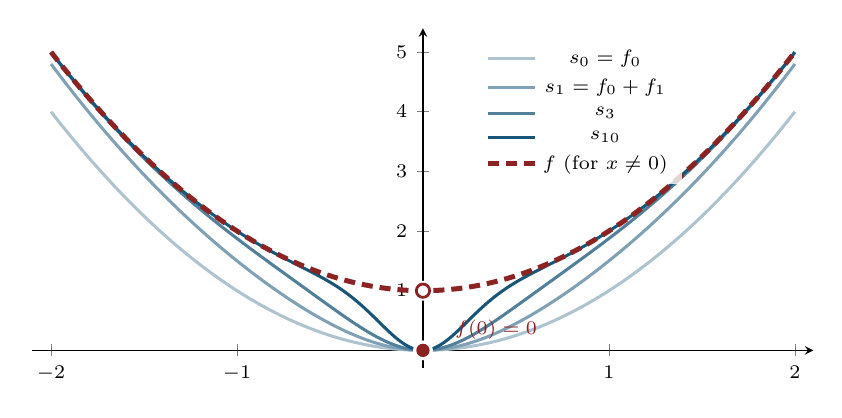
\begin{tikzpicture}
    \begin{axis}[
      width=11.5cm, height=5.9cm,
      axis lines=middle,
      xmin=-2.1, xmax=2.1, ymin=-0.3, ymax=5.4,
      xtick={-2,-1,1,2}, ytick={1,2,3,4,5},
      tick label style={font=\scriptsize},
      legend style={font=\scriptsize, at={(0.7,0.97)}, anchor=north,
        draw=none, fill=white, fill opacity=0.8, text opacity=1},
      clip=false,
    ]
      % partial sums s_N(x) = (1+x^2)(1 - (1+x^2)^(-(N+1)))
      \addplot[defcolor!35, line width=1.1pt, domain=-2:2, samples=200]
        {(1+x^2)*(1 - (1+x^2)^(-1))};
      \addlegendentry{$s_0 = f_0$}
      \addplot[defcolor!55, line width=1.1pt, domain=-2:2, samples=200]
        {(1+x^2)*(1 - (1+x^2)^(-2))};
      \addlegendentry{$s_1 = f_0 + f_1$}
      \addplot[defcolor!75, line width=1.1pt, domain=-2:2, samples=200]
        {(1+x^2)*(1 - (1+x^2)^(-4))};
      \addlegendentry{$s_3$}
      \addplot[defcolor, line width=1.1pt, domain=-2:2, samples=300]
        {(1+x^2)*(1 - (1+x^2)^(-11))};
      \addlegendentry{$s_{10}$}
      \addplot[thmcolor, line width=1.8pt, dash pattern=on 4pt off 2.5pt, domain=-2:2, samples=120]
        {1+x^2};
      \addlegendentry{$f$ (for $x \neq 0$)}
      \opendotpt{thmcolor}{(axis cs:0,1)}
      \dotpt{thmcolor}{(axis cs:0,0)}
      \node[thmcolor, font=\scriptsize, anchor=west] at (axis cs:0.12,0.35) {$f(0) = 0$};
    \end{axis}
  \end{tikzpicture}
  \end{center}

  \note{
    In the picture, the blue curves are the partial sums "s" sub
    capital "N", the sum of the terms "f" sub 0 through "f" sub
    capital "N", for capital "N" equal to 0, 1, 3, and 10, in
    increasingly dark blue. Each partial sum is a continuous function, and each
    passes through the origin, because every term vanishes at "x"
    equals 0. The dashed red curve is the parabola 1 plus "x" squared,
    the sum of the series for "x" not equal to 0. As capital "N"
    grows, the blue curves hug the red parabola more and more closely,
    but near the origin each of them has to dive down to 0, and the
    dip becomes narrower and narrower. In the limit the dip shrinks to
    a single point: the open red circle at height 1 is not a value of
    "f", while the filled red dot at the origin is "f" of 0. The hole
    in the limit function is the discontinuity. Notice that the
    convergence is slow near 0 and fast far from 0, exactly the
    loophole we identified earlier. On to Example 7.4.
  }
\end{frame}
}

{
\usebackgroundtemplate{%
  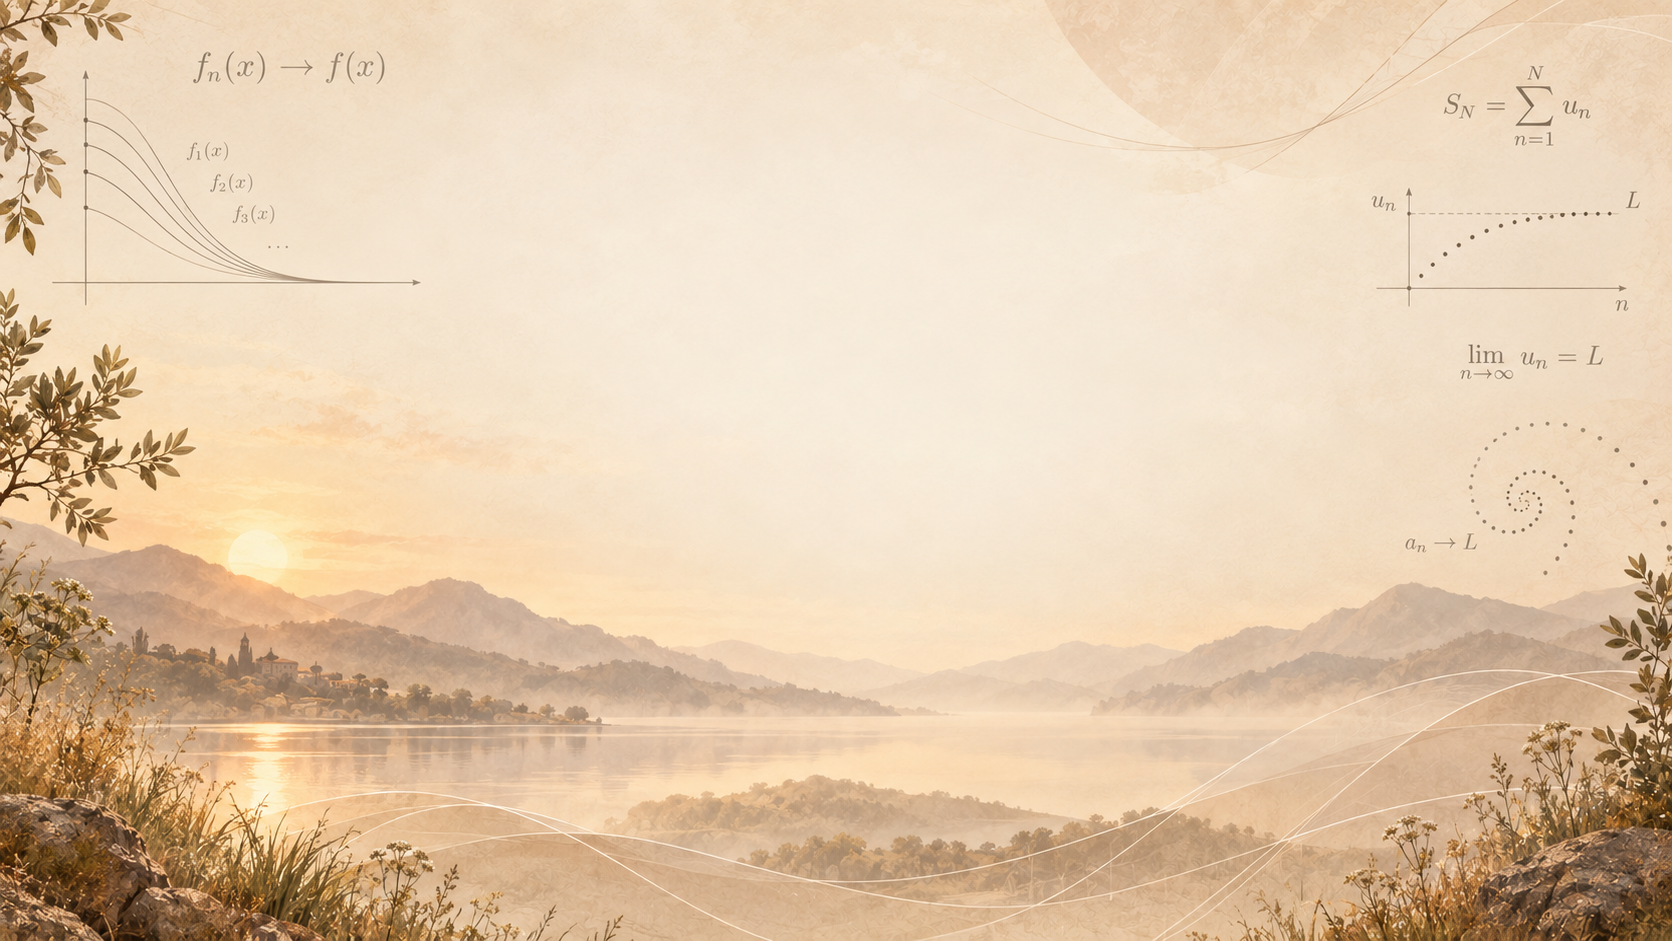
\includegraphics[width=\paperwidth,height=\paperheight,keepaspectratio=false]{chapter_07_bg_06.png}%
}
\section{Example 7.4: A Non-Integrable Limit}

% --- Build 1/2 ---
\begin{frame}{Example 7.4: The Inner Limit}
  \begin{exblock}{Example 7.4}
    For $m = 1, 2, 3, \dots$, put
    \[
      f_m(x) = \lim_{n \to \infty} (\cos\, m!\,\pi x)^{2n}.
    \]
  \end{exblock}

  \note{
    Example 7.4 is built from two limits taken one after the other.
    First, for each positive integer "m", define "f" sub "m" of "x" as
    the limit as "n" goes to infinity of cosine of "m" factorial times
    pi times "x", raised to the power 2 "n". The exponent is even so
    that the powers are never negative; in particular, when the cosine
    equals minus 1, the powers are all equal to 1 instead of
    alternating in sign. Let's see what this inner limit is.
  }
\end{frame}

% --- Build 2/2 ---
\begin{frame}{Example 7.4: The Inner Limit}
  \begin{exblock}{Example 7.4}
    For $m = 1, 2, 3, \dots$, put
    \[
      f_m(x) = \lim_{n \to \infty} (\cos\, m!\,\pi x)^{2n}.
    \]
  \end{exblock}
  \begin{hlbox}

  \begin{itemize}
    \item If $m!\,x$ is an \alert{integer}: $\cos(m!\,\pi x) = \pm 1$, so
      $(\cos m!\,\pi x)^{2n} = 1$ for all $n$, hence $\boxed{f_m(x) = 1}$
    \item Otherwise: $|\cos(m!\,\pi x)| < 1$, so
      $(\cos m!\,\pi x)^{2n} \to 0$, hence $\boxed{f_m(x) = 0}$
  \end{itemize}

  \vspace{0.2em}
  So $f_m$ equals $1$ exactly on the discrete set\\
  $\{x : m!\,x \in \mathbb{Z}\} = \{k/m! : k \in \mathbb{Z}\}$ and $0$ elsewhere.
  \end{hlbox}

\note{
    There are two cases. If "m" factorial times "x" is an integer,
    then the cosine of an integer multiple of pi is plus or minus 1,
    and raising it to an even power gives exactly 1 for every "n". So
    "f" sub "m" of "x" equals 1. Otherwise the cosine has absolute
    value strictly less than 1, and its powers tend to 0, so "f" sub
    "m" of "x" equals 0. The formula at the bottom summarizes this:
    "f" sub "m" is 1 at the points where "m" factorial times "x" is an
    integer, that is, at the multiples of 1 over "m" factorial, and 0
    everywhere else. Each "f" sub "m" is already a rather spiky
    function, but it is 1 only on a discrete set of equally spaced
    points. Now we take the outer limit.
  }
\end{frame}

% --- Build 1/3 ---
\begin{frame}{Example 7.4: The Outer Limit}

  \begin{hlbox}  Recall: $f_m(x) = 1$ if $m!\,x \in \mathbb{Z}$, and $f_m(x) = 0$ otherwise.
  Now let
  \[
    f(x) = \lim_{m \to \infty} f_m(x).
  \]
  \end{hlbox}

\note{
    Recalling the inner limit: "f" sub "m" of "x" is 1 when "m"
    factorial times "x" is an integer, and 0 otherwise. Now define "f"
    of "x" as the limit of "f" sub "m" of "x" as "m" goes to infinity.
    To evaluate it we distinguish irrational and rational "x".
  }
\end{frame}

% --- Build 2/3 ---
\begin{frame}{Example 7.4: The Outer Limit}

  \begin{hlbox}  Recall: $f_m(x) = 1$ if $m!\,x \in \mathbb{Z}$, and $f_m(x) = 0$ otherwise.
  Now let
  \[
    f(x) = \lim_{m \to \infty} f_m(x).
  \]

  \begin{itemize}
    \item $x$ \alert{irrational}: $m!\,x$ is never an integer, so $f_m(x) = 0$
      for every $m$; hence $f(x) = 0$
  \end{itemize}
  \end{hlbox}

\note{
    If "x" is irrational, then "m" factorial times "x" is irrational
    too, so it is never an integer. Therefore "f" sub "m" of "x" is 0
    for every "m", and the limit "f" of "x" is 0. Now the rational
    case.
  }
\end{frame}

% --- Build 3/3 ---
\begin{frame}{Example 7.4: The Outer Limit}

  \begin{hlbox}  Recall: $f_m(x) = 1$ if $m!\,x \in \mathbb{Z}$, and $f_m(x) = 0$ otherwise.
  Now let
  \[
    f(x) = \lim_{m \to \infty} f_m(x).
  \]

  \begin{itemize}
    \item $x$ \alert{irrational}: $m!\,x$ is never an integer, so $f_m(x) = 0$
      for every $m$; hence $f(x) = 0$
    \item $x$ \alert{rational}, $x = p/q$ with integers $p, q$: for $m \geq q$,
      $m!$ is divisible by $q$, so $m!\,x \in \mathbb{Z}$ and $f_m(x) = 1$;
      hence $f(x) = 1$
  \end{itemize}
  \end{hlbox}

\note{
    If "x" is rational, write it as "p" over "q" with integers "p" and
    "q". As soon as "m" is at least "q", the factorial "m" factorial
    contains "q" as a factor, so "m" factorial times "p" over "q" is
    an integer. Therefore "f" sub "m" of "x" equals 1 for all "m"
    from "q" onward, and the limit "f" of "x" is 1. This is the reason
    for the factorial in the formula: it guarantees that every
    denominator is eventually swallowed. Let's record the result.
  }
\end{frame}

% --- Build 1/3 ---
\begin{frame}{Example 7.4: An Everywhere Discontinuous Limit}

  \begin{hlbox}  \begin{equation}
    \lim_{m \to \infty}\, \lim_{n \to \infty} (\cos\, m!\,\pi x)^{2n}
    = \begin{cases} 0 & (x \text{ irrational}), \\ 1 & (x \text{ rational}). \end{cases} \tag{8}
  \end{equation}

  \vspace{0.4em}
  \begin{itemize}
    \item Every $(\cos m!\,\pi x)^{2n}$ is \emph{continuous}, indeed infinitely
      differentiable
  \end{itemize}
  \end{hlbox}

\note{
    Equation 8 is the result: the iterated limit is 0 at irrational
    "x" and 1 at rational "x". This is the famous Dirichlet function.
    Let's appreciate what happened. Each function we started from,
    cosine of "m" factorial times pi times "x", raised to an even power, is not
    only continuous but infinitely differentiable; it is about as
    nice as a function can be. Two limits later, look at what we get.
  }
\end{frame}

% --- Build 2/3 ---
\begin{frame}{Example 7.4: An Everywhere Discontinuous Limit}

  \begin{hlbox}  \begin{equation}
    \lim_{m \to \infty}\, \lim_{n \to \infty} (\cos\, m!\,\pi x)^{2n}
    = \begin{cases} 0 & (x \text{ irrational}), \\ 1 & (x \text{ rational}). \end{cases} \tag{8}
  \end{equation}

  \vspace{0.4em}
  \begin{itemize}
    \item Every $(\cos m!\,\pi x)^{2n}$ is \emph{continuous}, indeed infinitely
      differentiable
    \item The limit $f$ is \alert{discontinuous at every point}: rationals and
      irrationals are both dense
  \end{itemize}
  \end{hlbox}

\note{
    The limit "f" is discontinuous at every single point. The reason
    is that both the rationals and the irrationals are dense: every
    interval, no matter how short, contains points where "f" is 1 and
    points where "f" is 0, so "f" cannot settle down near any point.
    Compare this with Example 7.3, where the sum was discontinuous at
    just one point. Here continuity is lost everywhere. And it gets
    worse.
  }
\end{frame}

% --- Build 3/3 ---
\begin{frame}{Example 7.4: An Everywhere Discontinuous Limit}

  \begin{hlbox}  \begin{equation}
    \lim_{m \to \infty}\, \lim_{n \to \infty} (\cos\, m!\,\pi x)^{2n}
    = \begin{cases} 0 & (x \text{ irrational}), \\ 1 & (x \text{ rational}). \end{cases} \tag{8}
  \end{equation}

  \vspace{0.4em}
  \begin{itemize}
    \item Every $(\cos m!\,\pi x)^{2n}$ is \emph{continuous}, indeed infinitely
      differentiable
    \item The limit $f$ is \alert{discontinuous at every point}: rationals and
      irrationals are both dense
    \item $f$ is \alert{not Riemann-integrable} on any $[a, b]$
      (Exercise 4, Chap.\ 6): every upper sum is $b - a$, every lower sum is $0$
  \end{itemize}
  \end{hlbox}

\note{
    The function "f" is not Riemann integrable on any interval. This
    was Exercise 4 of Chapter 6: on every subinterval of a partition
    the supremum of "f" is 1 and the infimum is 0, so every upper sum
    equals the length "b" minus "a" and every lower sum equals 0, and
    the two never meet. So a pointwise limit of smooth functions can
    fail to be integrable at all; the question "is the integral of
    the limit equal to the limit of the integrals" does not even make
    sense here. Let's see the pictures that build this monster.
  }
\end{frame}

\begin{frame}[c]{Example 7.4: Spikes That Multiply}
  \begin{columns}[T]
    \begin{column}{0.56\textwidth}
      \begin{center}
      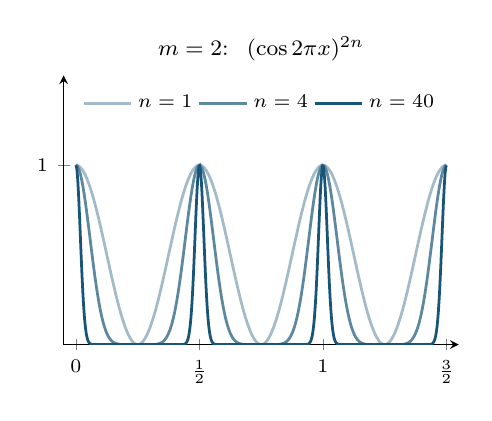
\begin{tikzpicture}
        \begin{axis}[
          width=6.6cm, height=5.0cm,
          axis lines=left,
          xmin=-0.05, xmax=1.55, ymin=0, ymax=1.5,
          xtick={0,0.5,1,1.5}, xticklabels={$0$,$\tfrac12$,$1$,$\tfrac32$},
          ytick={1},
          tick label style={font=\scriptsize},
          title={\footnotesize $m = 2$: \ $(\cos 2\pi x)^{2n}$},
          title style={yshift=-1ex},
          legend style={font=\scriptsize, at={(0.5,0.97)}, anchor=north,
            draw=none, fill=white, fill opacity=0.8, text opacity=1, legend columns=3},
        ]
          \addplot[defcolor!40, line width=1pt, domain=0:1.5, samples=300]
            {(cos(deg(2*pi*x))^2)^1};
          \addlegendentry{$n=1$}
          \addplot[defcolor!70, line width=1pt, domain=0:1.5, samples=400]
            {(cos(deg(2*pi*x))^2)^4};
          \addlegendentry{$n=4$}
          \addplot[defcolor, line width=1pt, domain=0:1.5, samples=600]
            {(cos(deg(2*pi*x))^2)^40};
          \addlegendentry{$n=40$}
        \end{axis}
      \end{tikzpicture}
      \end{center}
    \end{column}
    \begin{column}{0.44\textwidth}
      \vspace{0.6em}
      \begin{center}
      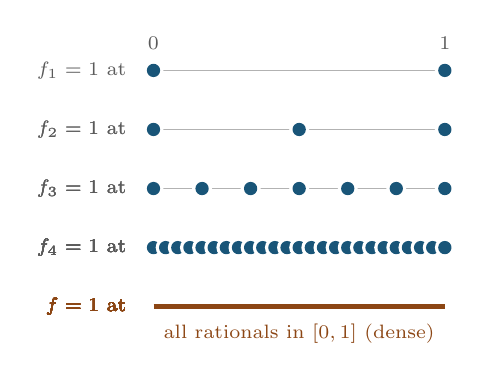
\begin{tikzpicture}[x=3.7cm, y=1cm, font=\scriptsize]
        \node[anchor=east, remcolor] at (-0.06,0) {$f_1 = 1$ at};
        \draw[gray!60] (0,0) -- (1,0);
        \foreach \x in {0,1} \dotpt{defcolor}{(\x,0)}
        \node[anchor=east, remcolor] at (-0.06,-0.75) {$f_2 = 1$ at};
        \draw[gray!60] (0,-0.75) -- (1,-0.75);
        \foreach \x in {0,0.5,1} \dotpt{defcolor}{(\x,-0.75)}
        \node[anchor=east, remcolor] at (-0.06,-1.5) {$f_3 = 1$ at};
        \draw[gray!60] (0,-1.5) -- (1,-1.5);
        \foreach \x in {0,0.1667,0.3333,0.5,0.6667,0.8333,1} \dotpt{defcolor}{(\x,-1.5)}
        \node[anchor=east, remcolor] at (-0.06,-2.25) {$f_4 = 1$ at};
        \draw[gray!60] (0,-2.25) -- (1,-2.25);
        \foreach \i in {0,...,24} \dotpt{defcolor}{(\i/24,-2.25)}
        \node[anchor=east, mAccent] at (-0.06,-3.0) {$f = 1$ at};
        \draw[mAccent, line width=1.6pt] (0,-3.0) -- (1,-3.0);
        \node[mAccent, anchor=north] at (0.5,-3.1) {all rationals in $[0,1]$ (dense)};
        \node[remcolor, anchor=north] at (0,0.55) {$0$};
        \node[remcolor, anchor=north] at (1,0.55) {$1$};
      \end{tikzpicture}
      \end{center}
    \end{column}
  \end{columns}

  \note{
    Two pictures. On the left, fix "m" equals 2, so "m" factorial is
    2, and plot cosine of 2 pi times "x", raised to the power 2 "n", for
    "n" equal to 1, 4, and 40, in increasingly dark blue. For "n" equals 1 we see
    gentle humps of height 1 at 0, one half, 1, and three halves, the
    points where 2 "x" is an integer. As "n" grows the humps become
    thin spikes, and in the limit only the spike tips survive: "f" sub
    2 is 1 at the multiples of one half and 0 elsewhere. On the right,
    each row of dots shows where "f" sub "m" equals 1 on the interval
    from 0 to 1. For "m" equals 1, only the integers 0 and 1. For "m"
    equals 2, also one half. For "m" equals 3, the multiples of one
    sixth. For "m" equals 4, the multiples of one twenty fourth, and
    so on: the set of ones grows with "m", because "m" factorial picks
    up more and more divisors. The orange line at the bottom is the
    limit: "f" equals 1 on all rationals, which are dense, and 0 on
    the irrationals, which are also dense. On to derivatives.
  }
\end{frame}
}

{
\usebackgroundtemplate{%
  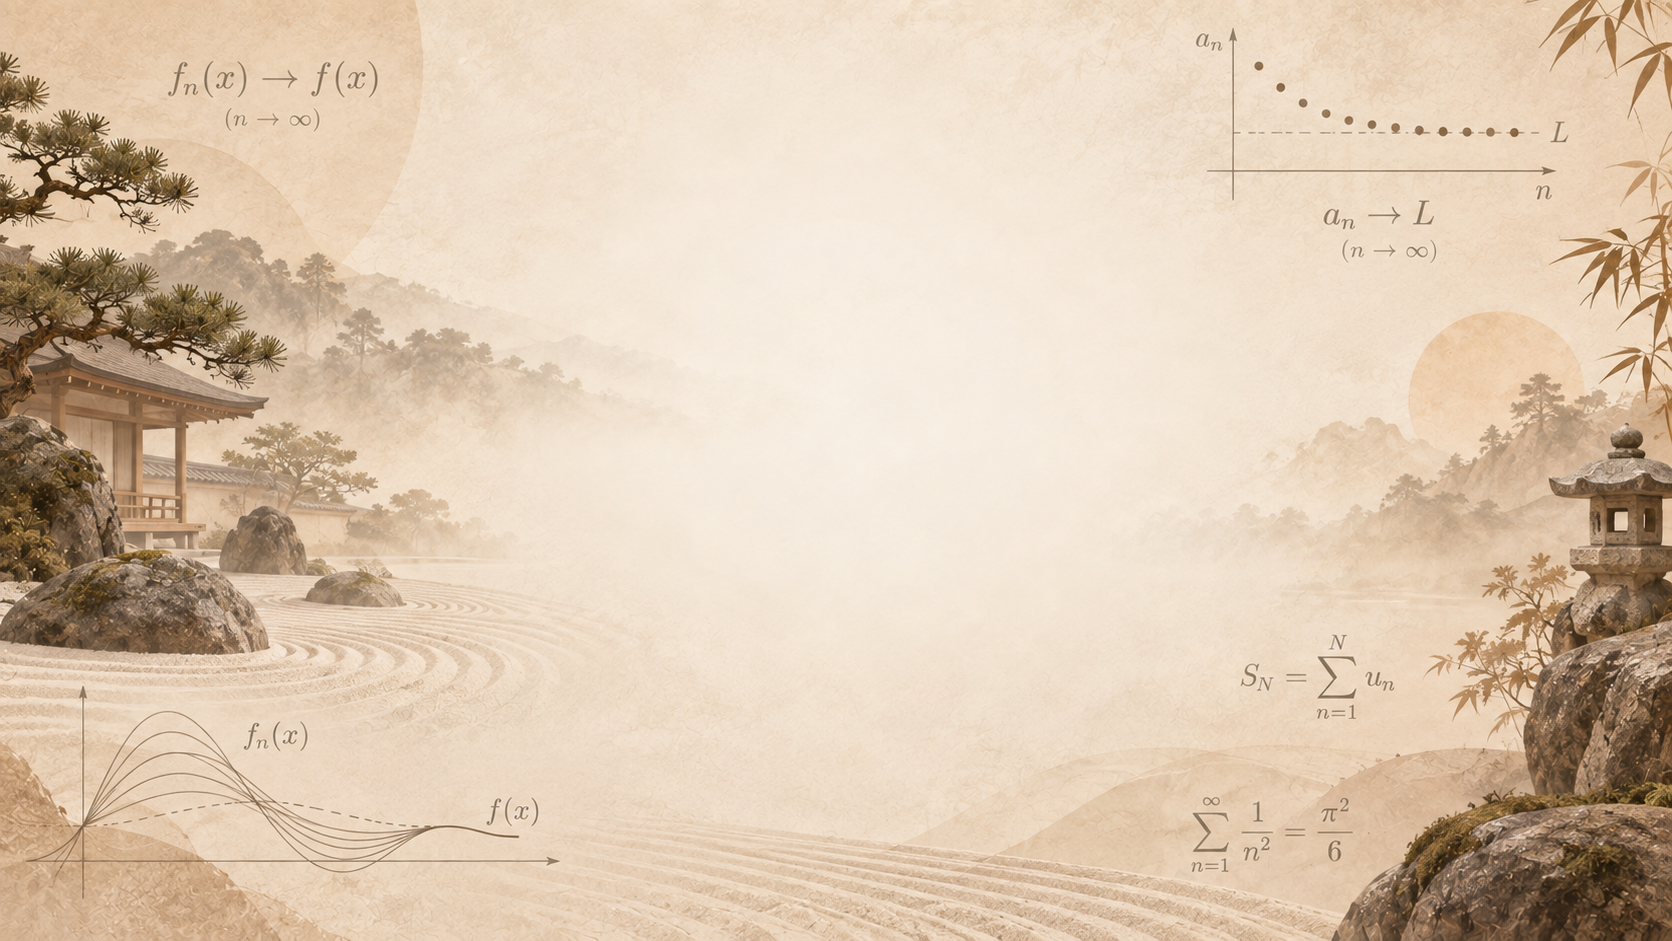
\includegraphics[width=\paperwidth,height=\paperheight,keepaspectratio=false]{chapter_07_bg_07.png}%
}
\section{Example 7.5: Derivatives}

% --- Build 1/3 ---
\begin{frame}{Example 7.5: Derivatives Need Not Converge}
  \begin{exblock}{Example 7.5}
    For real $x$ and $n = 1, 2, 3, \dots$, let
    \begin{equation}
      f_n(x) = \frac{\sin nx}{\sqrt{n}}. \tag{9}
    \end{equation}
  \end{exblock}
  \begin{hlbox}

  \vspace{0.2em}
  Since $|f_n(x)| \leq 1/\sqrt{n}$ for \emph{every} $x$:\\
  $f(x) = \lim_{n \to \infty} f_n(x) = 0$, \quad so \quad $f'(x) = 0$.
  \end{hlbox}

\note{
    Example 7.5 concerns derivatives. Let "f" sub "n" of "x" be sine
    of "n" times "x" divided by the square root of "n"; that is equation 9.
    The sine is bounded by 1 in absolute value, so "f" sub "n" of "x"
    is bounded by 1 over the square root of "n", for every "x" at
    once. As "n" goes to infinity this bound tends to 0, so the limit
    function "f" is identically 0, and its derivative "f" prime is
    identically 0 as well. Note how well behaved this convergence is:
    the bound does not depend on "x". Now differentiate the "f" sub
    "n".
  }
\end{frame}

% --- Build 2/3 ---
\begin{frame}{Example 7.5: Derivatives Need Not Converge}
  \begin{exblock}{Example 7.5}
    For real $x$ and $n = 1, 2, 3, \dots$, let
    \begin{equation}
      f_n(x) = \frac{\sin nx}{\sqrt{n}}. \tag{9}
    \end{equation}
  \end{exblock}
  \begin{hlbox}

  \vspace{0.2em}
  Since $|f_n(x)| \leq 1/\sqrt{n}$ for \emph{every} $x$:\\
  $f(x) = \lim_{n \to \infty} f_n(x) = 0$, \quad so \quad $f'(x) = 0$.

  \vspace{0.2em}
  But \quad $f_n'(x) = \sqrt{n}\,\cos nx$, \quad e.g.\
  $f_n'(0) = \sqrt{n} \to +\infty$, \quad whereas $f'(0) = 0$.
  \end{hlbox}

\note{
    Differentiating equation 9 by the chain rule, the derivative of
    sine of "n" times "x" is "n" times cosine of "n" times "x", and
    dividing by the square root of "n" leaves the square root of "n"
    times cosine of "n" times "x". At "x" equals 0 the cosine is 1, so "f" sub "n" prime
    of 0 equals the square root of "n", which tends to plus infinity.
    Meanwhile "f" prime of 0 is 0. The derivatives do not merely fail
    to converge to the right thing; at "x" equals 0 they do not
    converge at all.
  }
\end{frame}

% --- Build 3/3 ---
\begin{frame}{Example 7.5: Derivatives Need Not Converge}
  \begin{exblock}{Example 7.5}
    For real $x$ and $n = 1, 2, 3, \dots$, let
    \begin{equation}
      f_n(x) = \frac{\sin nx}{\sqrt{n}}. \tag{9}
    \end{equation}
  \end{exblock}
  \begin{hlbox}

  \vspace{0.2em}
  Since $|f_n(x)| \leq 1/\sqrt{n}$ for \emph{every} $x$:\\
  $f(x) = \lim_{n \to \infty} f_n(x) = 0$, \quad so \quad $f'(x) = 0$.

  \vspace{0.2em}
  But \quad $f_n'(x) = \sqrt{n}\,\cos nx$, \quad e.g.\
  $f_n'(0) = \sqrt{n} \to +\infty$, \quad whereas $f'(0) = 0$.

  \vspace{0.2em}
  \begin{center}
    \alert{$\{f_n'\}$ does not converge to $f'$}, even though
    $f_n \to f$ with a bound $1/\sqrt{n}$ \emph{independent of $x$}\\
    (this is \emph{uniform} convergence, Section 7.2, and it is still not enough).
  \end{center}
  \end{hlbox}

\note{
    So the sequence of derivatives does not converge to the derivative
    of the limit. The remark in orange is worth dwelling on. Here the
    functions "f" sub "n" converge to "f" as nicely as one could ask:
    the error is at most 1 over the square root of "n" at every point
    simultaneously. In the next section this will be called uniform
    convergence. Yet the derivatives misbehave. The lesson is that
    differentiation is a delicate operation: small functions can have
    large derivatives if they oscillate fast enough. When we return to
    derivatives in Section 7.5, we will need hypotheses on the
    derivatives themselves, not just on the functions. Let's look at
    the graphs.
  }
\end{frame}

\begin{frame}[c]{Example 7.5: Small Functions, Steep Slopes}
  \begin{center}
  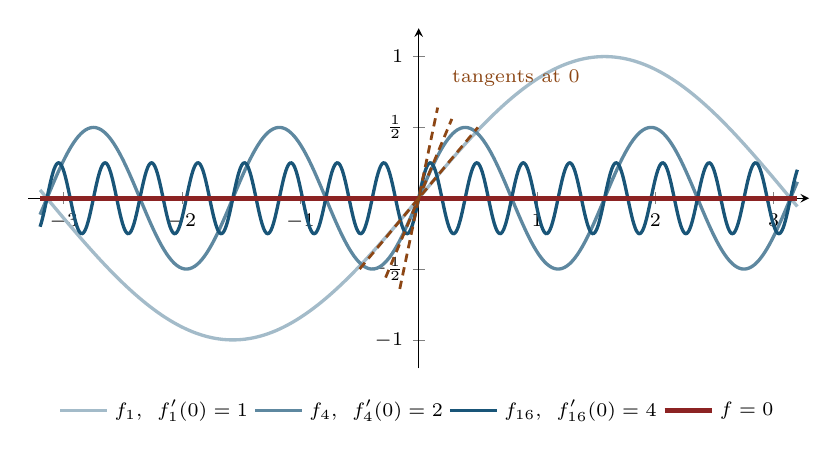
\begin{tikzpicture}
    \begin{axis}[
      width=11.5cm, height=5.9cm,
      axis lines=middle,
      xmin=-3.3, xmax=3.3, ymin=-1.2, ymax=1.2,
      xtick={-3,-2,-1,1,2,3}, ytick={-1,-0.5,0.5,1},
      yticklabels={$-1$,$-\tfrac12$,$\tfrac12$,$1$},
      tick label style={font=\scriptsize},
      legend style={font=\scriptsize, at={(0.5,-0.06)}, anchor=north,
        legend columns=4, draw=none, fill=white, fill opacity=0.8, text opacity=1},
      clip=false,
    ]
      \addplot[defcolor!40, line width=1.2pt, domain=-3.2:3.2, samples=200]
        {sin(deg(x))};
      \addlegendentry{$f_1$, \ $f_1'(0) = 1$}
      \addplot[defcolor!70, line width=1.2pt, domain=-3.2:3.2, samples=300]
        {sin(deg(4*x))/2};
      \addlegendentry{$f_4$, \ $f_4'(0) = 2$}
      \addplot[defcolor, line width=1.2pt, domain=-3.2:3.2, samples=700]
        {sin(deg(16*x))/4};
      \addlegendentry{$f_{16}$, \ $f_{16}'(0) = 4$}
      \addplot[thmcolor, line width=1.8pt, domain=-3.2:3.2, samples=2]
        {0};
      \addlegendentry{$f = 0$}
      % tangent lines at 0
      \draw[mAccent, line width=1pt, dash pattern=on 3pt off 2pt]
        (axis cs:-0.5,-0.5) -- (axis cs:0.5,0.5);
      \draw[mAccent, line width=1pt, dash pattern=on 3pt off 2pt]
        (axis cs:-0.28,-0.56) -- (axis cs:0.28,0.56);
      \draw[mAccent, line width=1pt, dash pattern=on 3pt off 2pt]
        (axis cs:-0.16,-0.64) -- (axis cs:0.16,0.64);
      \node[mAccent, font=\scriptsize, anchor=south west] at (axis cs:0.2,0.72) {tangents at $0$};
    \end{axis}
  \end{tikzpicture}
  \end{center}

  \note{
    The graphs show "f" sub 1, "f" sub 4, and "f" sub 16 in
    increasingly dark blue, and the limit "f" equals 0 as the thick
    red line along the axis. As "n" grows the amplitude shrinks, 1,
    then one half, then one fourth, so the curves squeeze toward the
    red line. But at the same time the oscillation gets faster, and
    the dashed orange tangent lines at the origin get steeper: slope
    1, then 2, then 4, the square roots of 1, 4, and 16. The functions
    flatten out while their derivatives at 0 blow up. This is the
    geometric content of Example 7.5: closeness of graphs says nothing
    about closeness of slopes. Finally, integrals.
  }
\end{frame}
}

{
\usebackgroundtemplate{%
  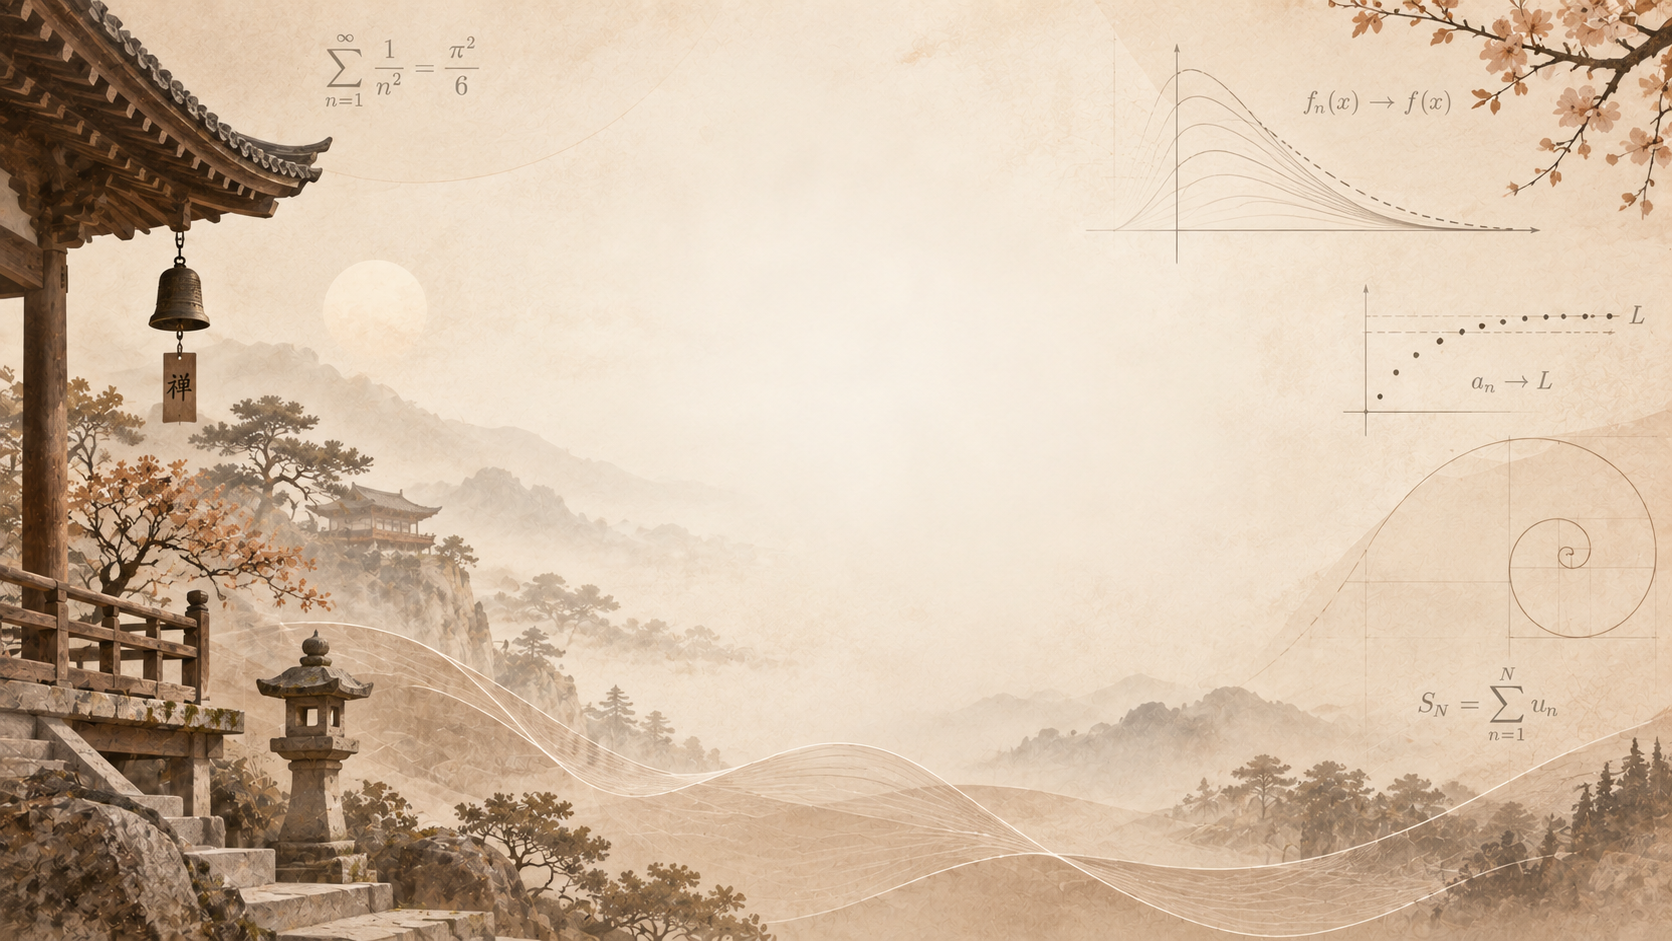
\includegraphics[width=\paperwidth,height=\paperheight,keepaspectratio=false]{chapter_07_bg_08.png}%
}
\section{Example 7.6: Integrals}

% --- Build 1/4 ---
\begin{frame}{Example 7.6: Integrals Need Not Converge}
  \begin{exblock}{Example 7.6}
    For $0 \leq x \leq 1$ and $n = 1, 2, 3, \dots$, let \quad
    $f_n(x) = n^2 x (1 - x^2)^n$. \hfill (10)
  \end{exblock}

  \note{
    Example 7.6 concerns integrals. On the closed interval from 0 to
    1, let "f" sub "n" of "x" be "n" squared times "x" times 1 minus
    "x" squared to the power "n"; that is equation 10. Each "f" sub
    "n" is a polynomial, so it is continuous and certainly integrable.
    We first find the pointwise limit.
  }
\end{frame}

% --- Build 2/4 ---
\begin{frame}{Example 7.6: Integrals Need Not Converge}
  \begin{exblock}{Example 7.6}
    For $0 \leq x \leq 1$ and $n = 1, 2, 3, \dots$, let \quad
    $f_n(x) = n^2 x (1 - x^2)^n$. \hfill (10)
  \end{exblock}
  \begin{hlbox}

  \textbf{Pointwise limit.} For $0 < x \leq 1$: $0 \leq 1 - x^2 < 1$, so
  $f_n(x) \to 0$ by Theorem 3.20(d); also $f_n(0) = 0$. Hence
  \begin{equation}
    \lim_{n \to \infty} f_n(x) = 0 \qquad (0 \leq x \leq 1). \tag{11}
  \end{equation}
  \end{hlbox}

\note{
    For "x" strictly between 0 and 1, or equal to 1, the number 1
    minus "x" squared lies in the half open interval from 0 to 1, so
    its powers decay geometrically. Recall Theorem 3.20 part "d": for
    "p" greater than 0 and any real alpha, "n" to the alpha divided by
    1 plus "p" to the "n" tends to 0. Geometric decay beats the
    polynomial factor "n" squared, so "f" sub "n" of "x" tends to 0.
    At "x" equals 0 every "f" sub "n" is 0 because of the factor "x".
    So the pointwise limit is 0 everywhere on the interval; that is
    equation 11. Now compute the integrals.
  }
\end{frame}

% --- Build 3/4 ---
\begin{frame}{Example 7.6: Integrals Need Not Converge}
  \begin{exblock}{Example 7.6}
    For $0 \leq x \leq 1$ and $n = 1, 2, 3, \dots$, let \quad
    $f_n(x) = n^2 x (1 - x^2)^n$. \hfill (10)
  \end{exblock}
  \begin{hlbox}

  \textbf{Pointwise limit.} For $0 < x \leq 1$: $0 \leq 1 - x^2 < 1$, so
  $f_n(x) \to 0$ by Theorem 3.20(d); also $f_n(0) = 0$. Hence
  \begin{equation}
    \lim_{n \to \infty} f_n(x) = 0 \qquad (0 \leq x \leq 1). \tag{11}
  \end{equation}

  \textbf{Integrals.} Substituting $u = 1 - x^2$, $du = -2x\,dx$:
  \[
    \int_0^1 x (1 - x^2)^n\,dx = \frac{1}{2}\int_0^1 u^n\,du = \frac{1}{2n + 2}.
  \]
  \end{hlbox}

\note{
    A simple calculation gives the integral of "x" times 1 minus "x"
    squared to the "n" over the interval. Substitute "u" equals 1
    minus "x" squared, whose derivative is minus 2 "x", so the factor
    "x" "d" "x" becomes minus one half "d" "u"; as "x" runs from 0 to
    1, "u" runs from 1 down to 0, and flipping the limits absorbs the
    minus sign. We are left with one half times the
    integral of "u" to the "n" from 0 to 1, which is one half times 1
    over "n" plus 1, that is, 1 over 2 "n" plus 2. Now multiply by "n"
    squared.
  }
\end{frame}

% --- Build 4/4 ---
\begin{frame}{Example 7.6: Integrals Need Not Converge}
  \begin{exblock}{Example 7.6}
    For $0 \leq x \leq 1$ and $n = 1, 2, 3, \dots$, let \quad
    $f_n(x) = n^2 x (1 - x^2)^n$. \hfill (10)
  \end{exblock}
  \begin{hlbox}

  \textbf{Pointwise limit.} For $0 < x \leq 1$: $0 \leq 1 - x^2 < 1$, so
  $f_n(x) \to 0$ by Theorem 3.20(d); also $f_n(0) = 0$. Hence
  \begin{equation}
    \lim_{n \to \infty} f_n(x) = 0 \qquad (0 \leq x \leq 1). \tag{11}
  \end{equation}

  \textbf{Integrals.} Substituting $u = 1 - x^2$, $du = -2x\,dx$; then, in spite of (11):
  \[
    \int_0^1 x (1 - x^2)^n\,dx = \tfrac{1}{2}\int_0^1 u^n\,du = \frac{1}{2n + 2},
    \quad
    \boxed{\int_0^1 f_n(x)\,dx = \frac{n^2}{2n + 2} \to +\infty.}
  \]
  \end{hlbox}

\note{
    Thus the integral of "f" sub "n" over the interval is "n" squared
    divided by 2 "n" plus 2, which behaves like "n" over 2 and tends
    to plus infinity, as shown in the box. So in spite of equation 11,
    which says the functions converge to 0 at every point, their
    integrals grow without bound. The integral of the limit is 0, but
    the limit of the integrals does not even exist as a finite number.
    One might object that this is only because the integrals blow up.
    Let's tame the example and see that the problem persists.
  }
\end{frame}

% --- Build 1/2 ---
\begin{frame}{Example 7.6 (continued): Both Finite, Still Unequal}

  \begin{hlbox}  Replace $n^2$ by $n$ in (10): \quad $f_n(x) = n\,x (1 - x^2)^n$ \quad $(0 \leq x \leq 1)$.

  \vspace{0.3em}
  Then (11) still holds: $\lim_{n\to\infty} f_n(x) = 0$ for $0 \leq x \leq 1$. But now
  \begin{align*}
    \lim_{n \to \infty} \int_0^1 f_n(x)\,dx
    &= \lim_{n \to \infty} \frac{n}{2n + 2} = \frac{1}{2},
  \end{align*}
  \end{hlbox}

\note{
    Replace "n" squared by "n" in equation 10, so that "f" sub "n" of
    "x" is "n" times "x" times 1 minus "x" squared to the "n". The
    argument for equation 11 is unchanged: geometric decay still beats
    the factor "n", so the pointwise limit is still 0. But the
    integral is now "n" divided by 2 "n" plus 2, which converges to
    one half. So the limit of the integrals is a perfectly finite
    number, one half. Compare it with the integral of the limit.
  }
\end{frame}

% --- Build 2/2 ---
\begin{frame}{Example 7.6 (continued): Both Finite, Still Unequal}

  \begin{hlbox}  Replace $n^2$ by $n$ in (10): \quad $f_n(x) = n\,x (1 - x^2)^n$ \quad $(0 \leq x \leq 1)$.

  \vspace{0.3em}
  Then (11) still holds: $\lim_{n\to\infty} f_n(x) = 0$ for $0 \leq x \leq 1$. But now
  \begin{align*}
    \lim_{n \to \infty} \int_0^1 f_n(x)\,dx
    &= \lim_{n \to \infty} \frac{n}{2n + 2} = \frac{1}{2}, \\
    \text{whereas}\qquad
    \int_0^1 \Big[\lim_{n \to \infty} f_n(x)\Big]\,dx &= \int_0^1 0\,dx = 0.
  \end{align*}

  \vspace{0.3em}
  \begin{center}
    \alert{The limit of the integral need not equal the integral of the
    limit, even if both are finite.}
  \end{center}
  \end{hlbox}

\note{
    The integral of the limit function is the integral of 0, which is
    0. So the limit of the integrals is one half, while the integral
    of the limit is 0. As the orange conclusion says, the limit of the
    integral need not equal the integral of the limit, even when both
    are finite. This is again an interchange of two limit processes,
    the integral, which is a limit of Riemann sums, and the limit in
    "n". Let's see the graphs to understand where the missing one half
    went.
  }
\end{frame}

\begin{frame}[c]{Example 7.6: The Escaping Bump}
  \begin{center}
  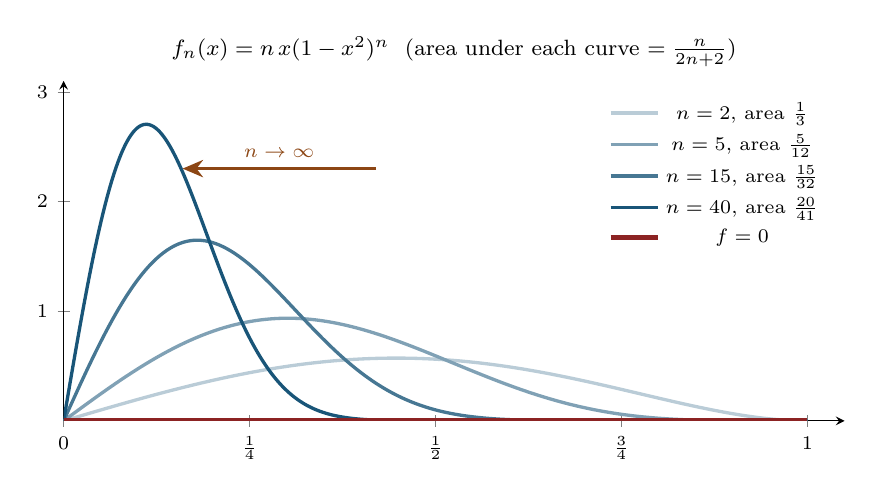
\begin{tikzpicture}
    \begin{axis}[
      width=11.5cm, height=5.9cm,
      axis lines=left,
      xmin=0, xmax=1.05, ymin=0, ymax=3.1,
      xtick={0,0.25,0.5,0.75,1}, xticklabels={$0$,$\tfrac14$,$\tfrac12$,$\tfrac34$,$1$},
      ytick={1,2,3},
      tick label style={font=\scriptsize},
      title={\footnotesize $f_n(x) = n\,x(1-x^2)^n$ \ (area under each curve $= \tfrac{n}{2n+2}$)},
      title style={yshift=-1ex},
      legend style={font=\scriptsize, at={(0.985,0.97)}, anchor=north east,
        draw=none, fill=white, fill opacity=0.8, text opacity=1},
    ]
      \addplot[defcolor!30, line width=1.2pt, domain=0:1, samples=200]
        {2*x*(1-x^2)^2};
      \addlegendentry{$n=2$, area $\tfrac13$}
      \addplot[defcolor!55, line width=1.2pt, domain=0:1, samples=200]
        {5*x*(1-x^2)^5};
      \addlegendentry{$n=5$, area $\tfrac5{12}$}
      \addplot[defcolor!80, line width=1.2pt, domain=0:1, samples=300]
        {15*x*(1-x^2)^15};
      \addlegendentry{$n=15$, area $\tfrac{15}{32}$}
      \addplot[defcolor, line width=1.2pt, domain=0:1, samples=400]
        {40*x*(1-x^2)^40};
      \addlegendentry{$n=40$, area $\tfrac{20}{41}$}
      \addplot[thmcolor, line width=1.8pt, domain=0:1, samples=2] {0};
      \addlegendentry{$f = 0$}
      \draw[guide, mAccent] (axis cs:0.42,2.3) -- (axis cs:0.16,2.3)
        node[midway, above, font=\scriptsize] {$n \to \infty$};
    \end{axis}
  \end{tikzpicture}
  \end{center}

  \note{
    The picture shows the tamed version, "n" times "x" times 1 minus
    "x" squared to the "n", for "n" equal to 2, 5, 15, and 40, in
    increasingly dark blue, together with the limit "f" equals 0 as
    the thick red line along the axis. Each curve is a bump: it starts
    at 0, rises to a peak, and decays to 0 at "x" equals 1. As "n"
    grows the bump gets taller and narrower, and it slides toward the
    left edge, as the orange arrow indicates. At any fixed "x" greater
    than 0 the bump eventually passes by and the values drop to 0,
    which is the pointwise convergence. But the area under the bump,
    listed in the legend, does not disappear; it increases toward one
    half. The mass escapes into an ever thinner region near 0, where
    the pointwise limit cannot see it. With "n" squared instead of "n"
    the bumps are "n" times taller and the area escapes to infinity.
    Let's summarize.
  }
\end{frame}
}

{
\usebackgroundtemplate{%
  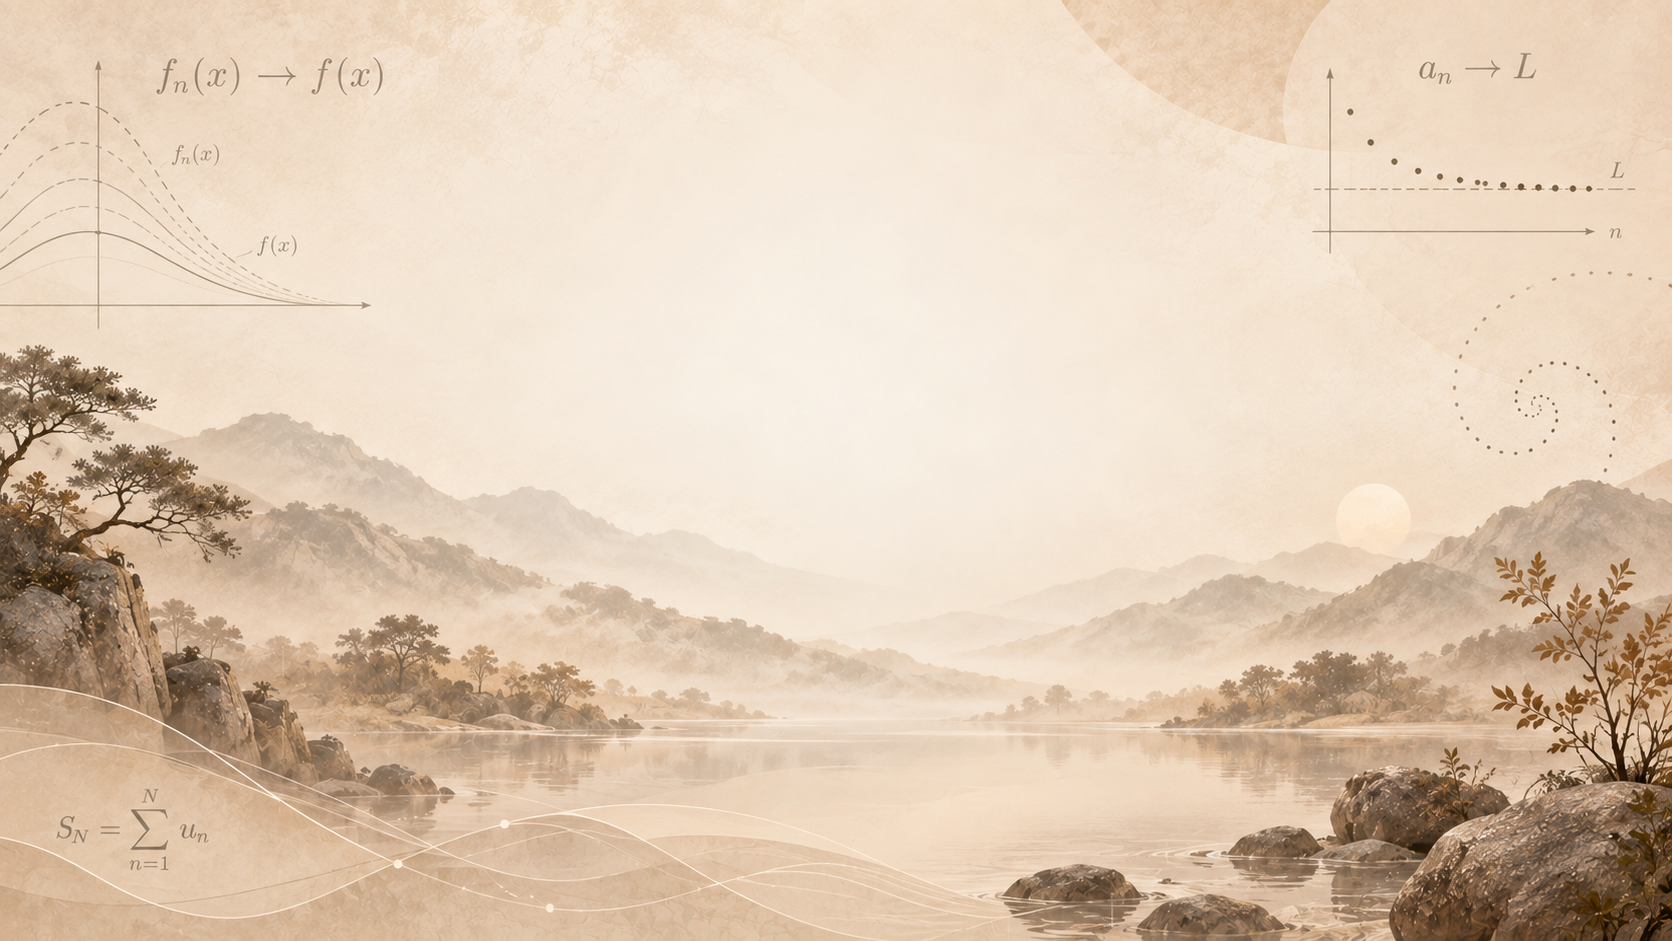
\includegraphics[width=\paperwidth,height=\paperheight,keepaspectratio=false]{chapter_07_bg_09.png}%
}
\section{Summary}

% --- Build 1/4 ---
\begin{frame}{Summary}

  \begin{hlbox}  \textbf{Key takeaways from this section:}
  \begin{itemize}
    \item \textbf{Definition 7.1:} $f_n \to f$ \alert{pointwise} on $E$ means
      $f(x) = \lim_n f_n(x)$ for each $x \in E$; likewise the \emph{sum} of a
      series. $N$ depends on $x$.
  \end{itemize}
  \end{hlbox}

\note{
    Let's review what we covered. First, Definition 7.1: a sequence of
    functions converges pointwise to "f" on capital "E" if at every
    point "x" the numbers "f" sub "n" of "x" converge to "f" of "x",
    and a series of functions converges to its sum in the same
    pointwise sense. We emphasized that the threshold capital "N" in
    the definition is allowed to depend on the point "x", so
    convergence can be fast at some points and slow at others. Next,
    the main problem.
  }
\end{frame}

% --- Build 2/4 ---
\begin{frame}{Summary}

  \begin{hlbox}  \textbf{Key takeaways from this section:}
  \begin{itemize}
    \item \textbf{Definition 7.1:} $f_n \to f$ \alert{pointwise} on $E$ means
      $f(x) = \lim_n f_n(x)$ for each $x \in E$; likewise the \emph{sum} of a
      series. $N$ depends on $x$.
    \item \textbf{Main problem:} are continuity, differentiability, integrability
      preserved under (1), (2)? Each asks whether \alert{two limits can be
      interchanged}, as in (3)
  \end{itemize}
  \end{hlbox}

\note{
    Second, the main problem: whether continuity, differentiability,
    and integrability of the "f" sub "n" are inherited by "f". We saw
    that each of these is a question about interchanging two limit
    processes. For continuity this is equation 3, which asks whether
    the limit in "t" and the limit in "n" may be swapped; the two
    routes around the square must lead to the same value. Third, the
    examples.
  }
\end{frame}

% --- Build 3/4 ---
\begin{frame}{Summary}

  \begin{hlbox}  \textbf{Key takeaways from this section:}
  \begin{itemize}
    \item \textbf{Definition 7.1:} $f_n \to f$ \alert{pointwise} on $E$ means
      $f(x) = \lim_n f_n(x)$ for each $x \in E$; likewise the \emph{sum} of a
      series. $N$ depends on $x$.
    \item \textbf{Main problem:} are continuity, differentiability, integrability
      preserved under (1), (2)? Each asks whether \alert{two limits can be
      interchanged}, as in (3)
    \item \textbf{Examples 7.2--7.6:} in general \alert{no}: iterated limits
      differ; continuous terms, discontinuous sum; non-integrable limit;
      $f_n' \not\to f'$; $\int f_n \not\to \int f$
  \end{itemize}
  \end{hlbox}

\note{
    Third, Examples 7.2 through 7.6 showed that in general the answer
    is no. The double sequence "m" over "m" plus "n" has iterated
    limits 1 and 0 depending on the order. A geometric series of
    continuous functions summed to a function with a hole at the
    origin. Two limits of powers of cosines produced the Dirichlet
    function, discontinuous everywhere and not Riemann integrable. The
    functions sine of "n" times "x" over root "n" converge to 0 while
    their derivatives at 0 blow up. And the escaping bumps "n" times
    "x" times 1 minus "x" squared to the "n" converge to 0 pointwise while their
    integrals converge to one half. Finally, where do we go from here?
  }
\end{frame}

% --- Build 4/4 ---
\begin{frame}{Summary}

  \begin{hlbox}  \textbf{Key takeaways from this section:}
  \begin{itemize}
    \item \textbf{Definition 7.1:} $f_n \to f$ \alert{pointwise} on $E$ means
      $f(x) = \lim_n f_n(x)$ for each $x \in E$; likewise the \emph{sum} of a
      series. $N$ depends on $x$.
    \item \textbf{Main problem:} are continuity, differentiability, integrability
      preserved under (1), (2)? Each asks whether \alert{two limits can be
      interchanged}, as in (3)
    \item \textbf{Examples 7.2--7.6:} in general \alert{no}: iterated limits
      differ; continuous terms, discontinuous sum; non-integrable limit;
      $f_n' \not\to f'$; $\int f_n \not\to \int f$
  \end{itemize}

  \vspace{0.3em}
  \textbf{Coming up next:} \alert{uniform convergence}: limits \emph{can} be interchanged.
  \end{hlbox}

\note{
    These examples show what can go wrong when limit processes are
    interchanged carelessly. In most of them the common thread is that
    pointwise convergence lets the speed of convergence vary from
    point to point, and the trouble hides where convergence is slow:
    near the hole in Example 7.3, at the rationals in Example 7.4, in
    the escaping bump in Example 7.6. In the next section we define a
    new mode of convergence, uniform convergence, which demands a
    single threshold capital "N" that works for all points of
    capital "E" at once. It is exactly what is needed to arrive at positive
    results: limits of continuous functions will be continuous, and
    integrals will pass to the limit. Example 7.5 is the warning that
    derivatives are different: there the convergence was already
    uniform, and the derivatives still misbehaved, so derivatives will
    need hypotheses of their own. See you next time.
  }
\end{frame}
}

\end{document}
